\subsection{Overview}

\begin{figure}[H]
    \centering
    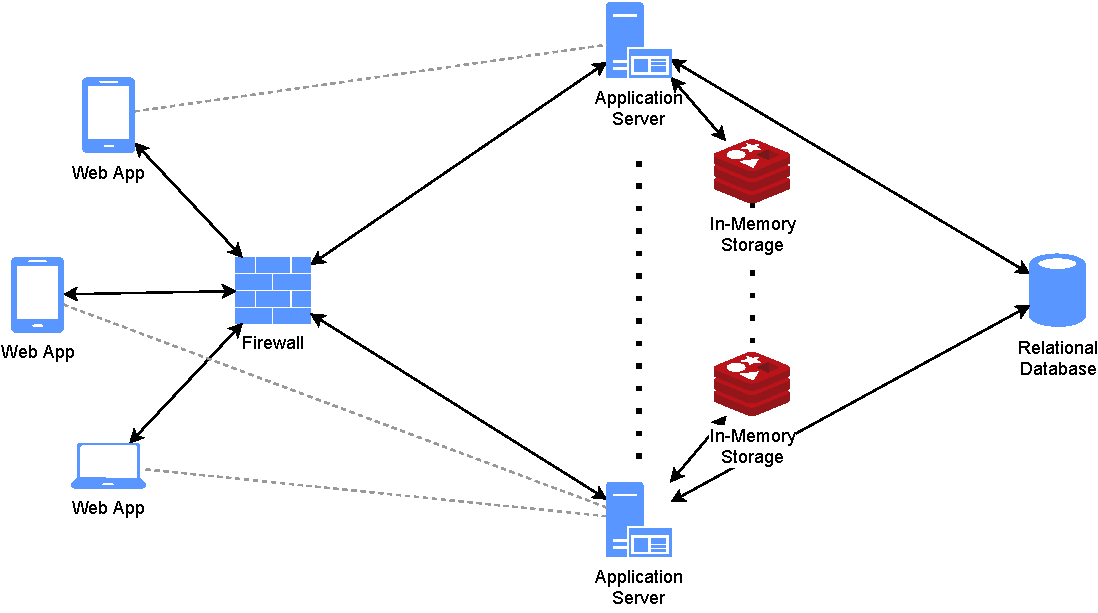
\includegraphics[width=.85\textwidth]{Images/overview.pdf}
    \caption{\label{fig:world_machine} Architecture overview}
\end{figure}
The figure above shows an high level representation of the \emph{CLup} system architecture.
Two parts can be easily distinguished, separated by the firewall: the Client Web Application and the Application Server with its data storage.
Further details on the System components and their interactions will be examined in the following sections.

\subsection{Component view}

\begin{figure}[H]
    \centering
    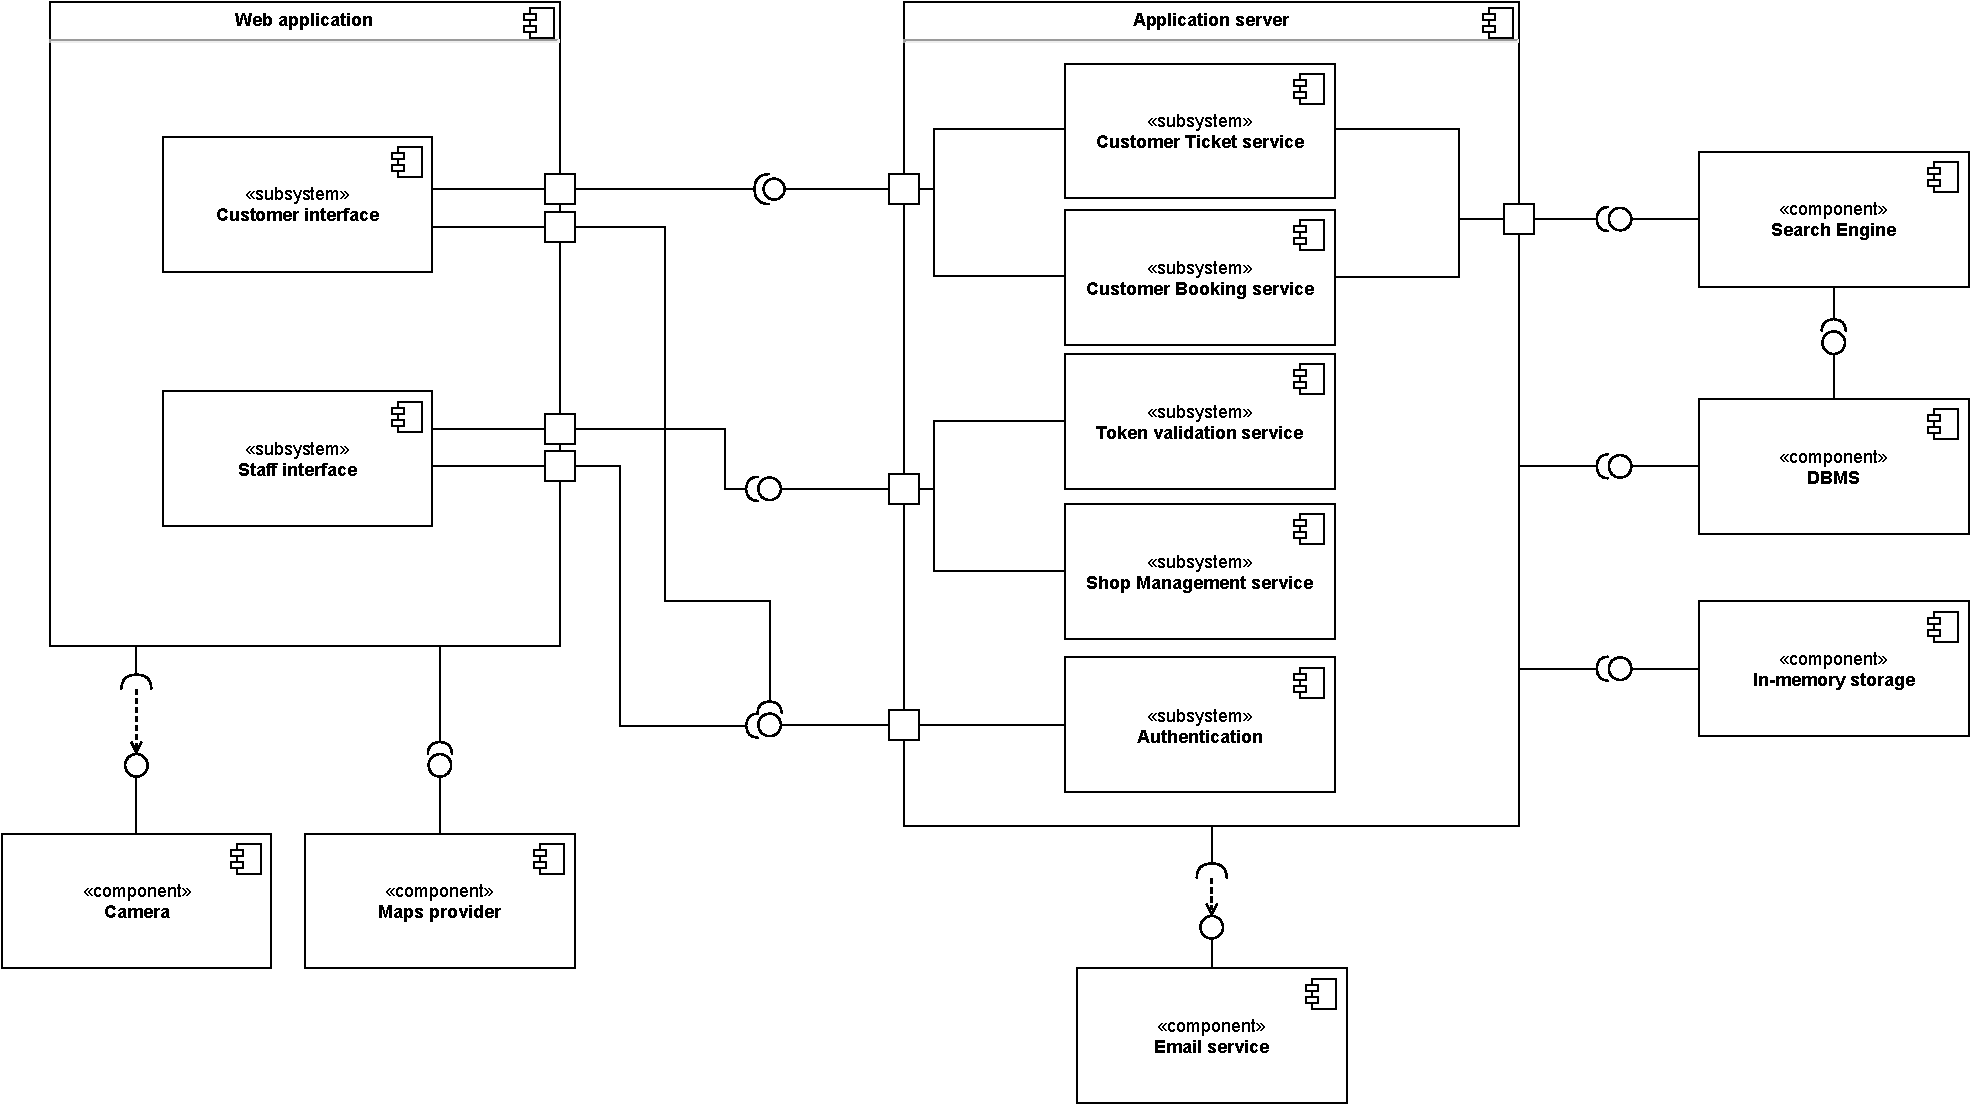
\includegraphics[width=.85\textwidth]{Images/component2.pdf}
    \caption{\label{fig:component_diagram} Component diagram of the full system}
\end{figure}

In this section, an UML component diagram shows the internal structure of the \emph{CLup} system. The architecture is simple, there are a small number of components and few external service providers. It can be divided in two higher level components: a Web Application and an Application Server, with the respective dependencies.
As for component dependencies, the Web application uses a Camera module to scan the QR codes, and it can use an optiona Map service provider to show directions. The Application server uses a DBMS, an in-memory data store and a search engine.
The relationships and interfaces between the components are represented through assembly connectors and delegation connectors.
A detailed description of the components is included in the following paragraphs:

\textbf{Web application}\\
\emph{CLup} is a distributed system, therefore part of the logic is included in the client. The Web Application client consists of two main components and some external interfaces:
\begin{itemize}
    \item \textbf{Customer interface} is what Customers use to interact with the service. It processes the inputs, transparently querying the application server with transformed data, and it transforms the repsonses into a user frierndly representation. The application guides the user through the creation of a Ticket or a Booking while performing input validation to reduce the workload on the application server. It can interface with a \emph{Maps provider} to display a Map with directions to the Shop.
    \item \textbf{Staff interface} is what the Staff uses to interact with the service. The behaviour is similar to that of the Customer interface, however the functionalities allow checking tokens and managing the shops. It interfaces with a \emph{Camera} to scan the QR codes associated with tokens
\end{itemize}

\textbf{Application server}\\
The application server is accessed through a REST API. Its internal structure follows the Actor model (\ref{sect:patterns}) so it can be seen as a set of components which have no shared state. The actors can be organized and seen as three groups based on their functions:
\begin{itemize}
    \item \textbf{Authentication} handles registrations and logins. It interfaces with the DBMS to validate and update credentials and with the Session Store to create and update Sessions. It can verify or update login credentials and authenticate a user Session.
    \item \textbf{Customer Ticket service} interface with the Search engine to allow users to find Shops. It uses Session storage to check authentication and update session data. It interacts with the DBMS to retrieve the persistent data necessary for the services. It allows users to create Tickets, search Shops and receive time estimates.
    \item \textbf{Customer Booking service} interface with the Search engine with the Ticket Service and has a similar policy to the Session storage and the DBMS. It computes the availability of Shop departments to decide whether to accept Booking requests.
    \item \textbf{Token validation service} It uses Session storage to check authentication and update session data. It interacts with the DBMS to retrieve the persistent data necessary for the services. It allows the Staff to validate Tokens. 
    \item \textbf{Shop Management service} interfaces with the DBMS. It allows the Managers to add and edit Shops, check tehir current status and occupancy.

\end{itemize}
\textbf{Application server external Interfaces}\\
The application server has interfaces for its internal components in the form of REST API. The web application can interact with the Application Server by sending HTTP queries to the endpoints described in the API (\ref{sect:api})

\textbf{Search Engine}\\ This component generates real-time search results to allow Customers to find a Shop by name.

\textbf{DBMS}\\ Stores the long term persistent data regarding Shops, Bookings, Tickets and Account data in a relational database.

\textbf{In-memory Session Store}\\ Keeps track of Sessions and stores data that should persist throughout the lifetime of a session. It provides a fast in-memory data structure that the Application server can use for non critical data to reduce the frequency of accesses to the relational database.

\textbf{Email service}\\ It provides the capability to send emails to new Customers to validate their email address.


\subsection{Deployment view}
The deployment view shows the organization of the distributed devices that make up the Clup service with a UML deployment diagram. The first tier is the \emph{Presentation tier}, represented by the web application. The web application can be accessed either through a web browser as a normal website, or installed on a smartphone as a \emph{Progressive Web App}. The middle tier, is the \emph{Logic tier}, composed of the application server running the Clup artifact, the reverse proxy serving static pages, and the Redis session store. The last tier is the \emph{Data tier} running a DBMS.
\begin{figure}[H]
    \centering
    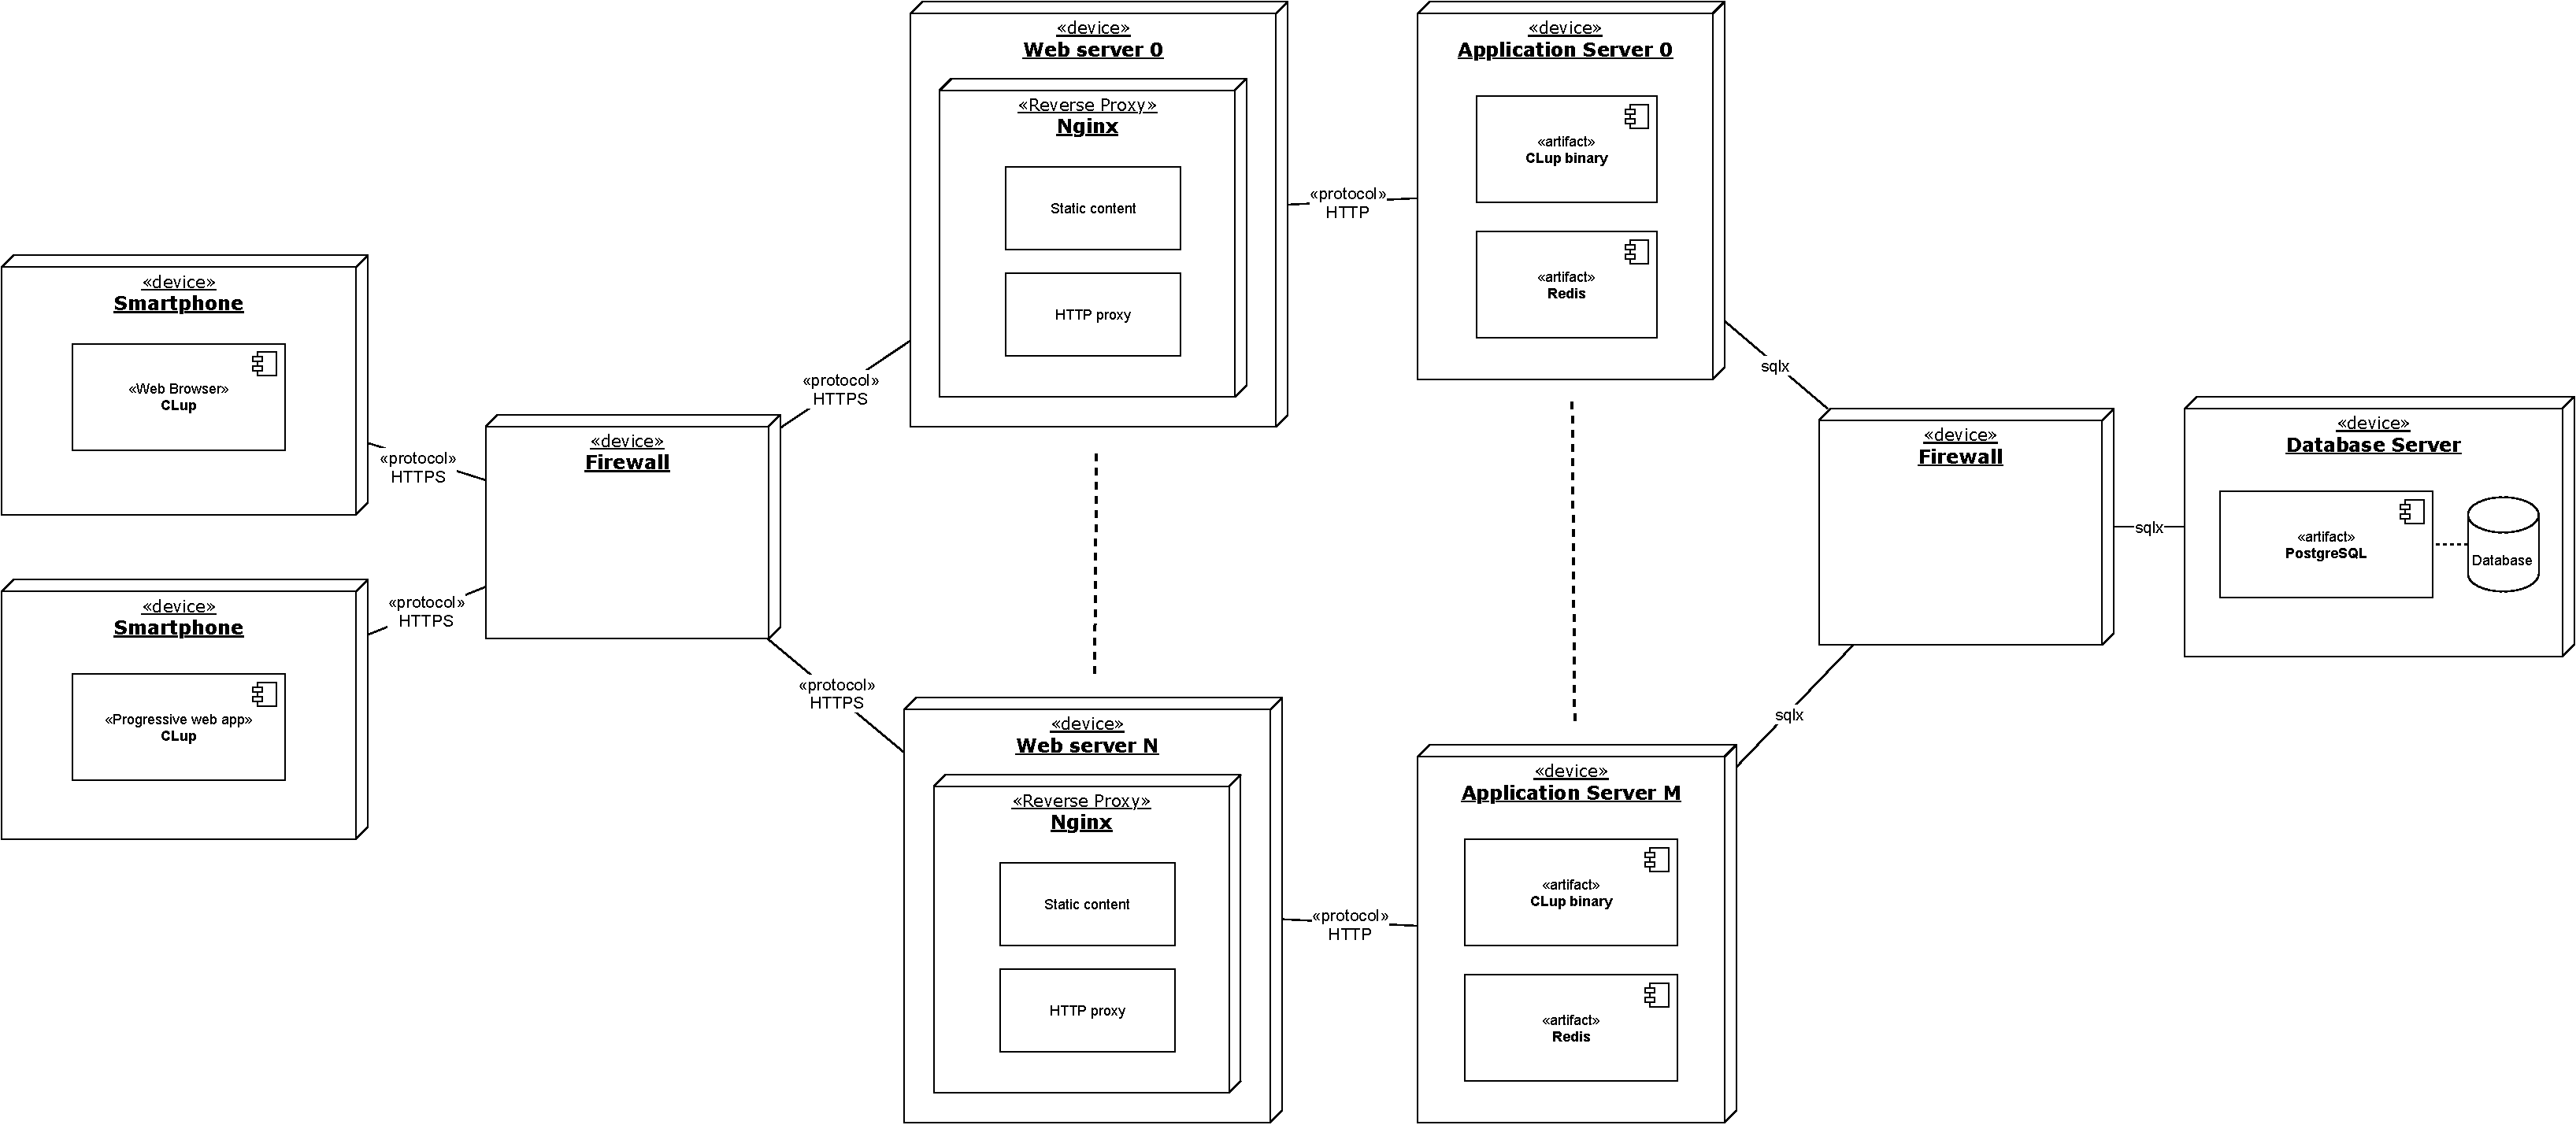
\includegraphics[width=1\textwidth]{Images/deployment-1.pdf}
    \caption{Deployment Diagram}
\end{figure}
CLup can also be deployed in a containerized environment as stated in the portability section of the RASD. This deployment scenario is easier to setup and adapts to many different device layouts. It can be deployed on a single machine running docker, a docker cluster or in the cloud. Configuring the service in a containerized environment is easier since installing dependencies and connecting components is automated.
\begin{figure}[H]
    \centering
    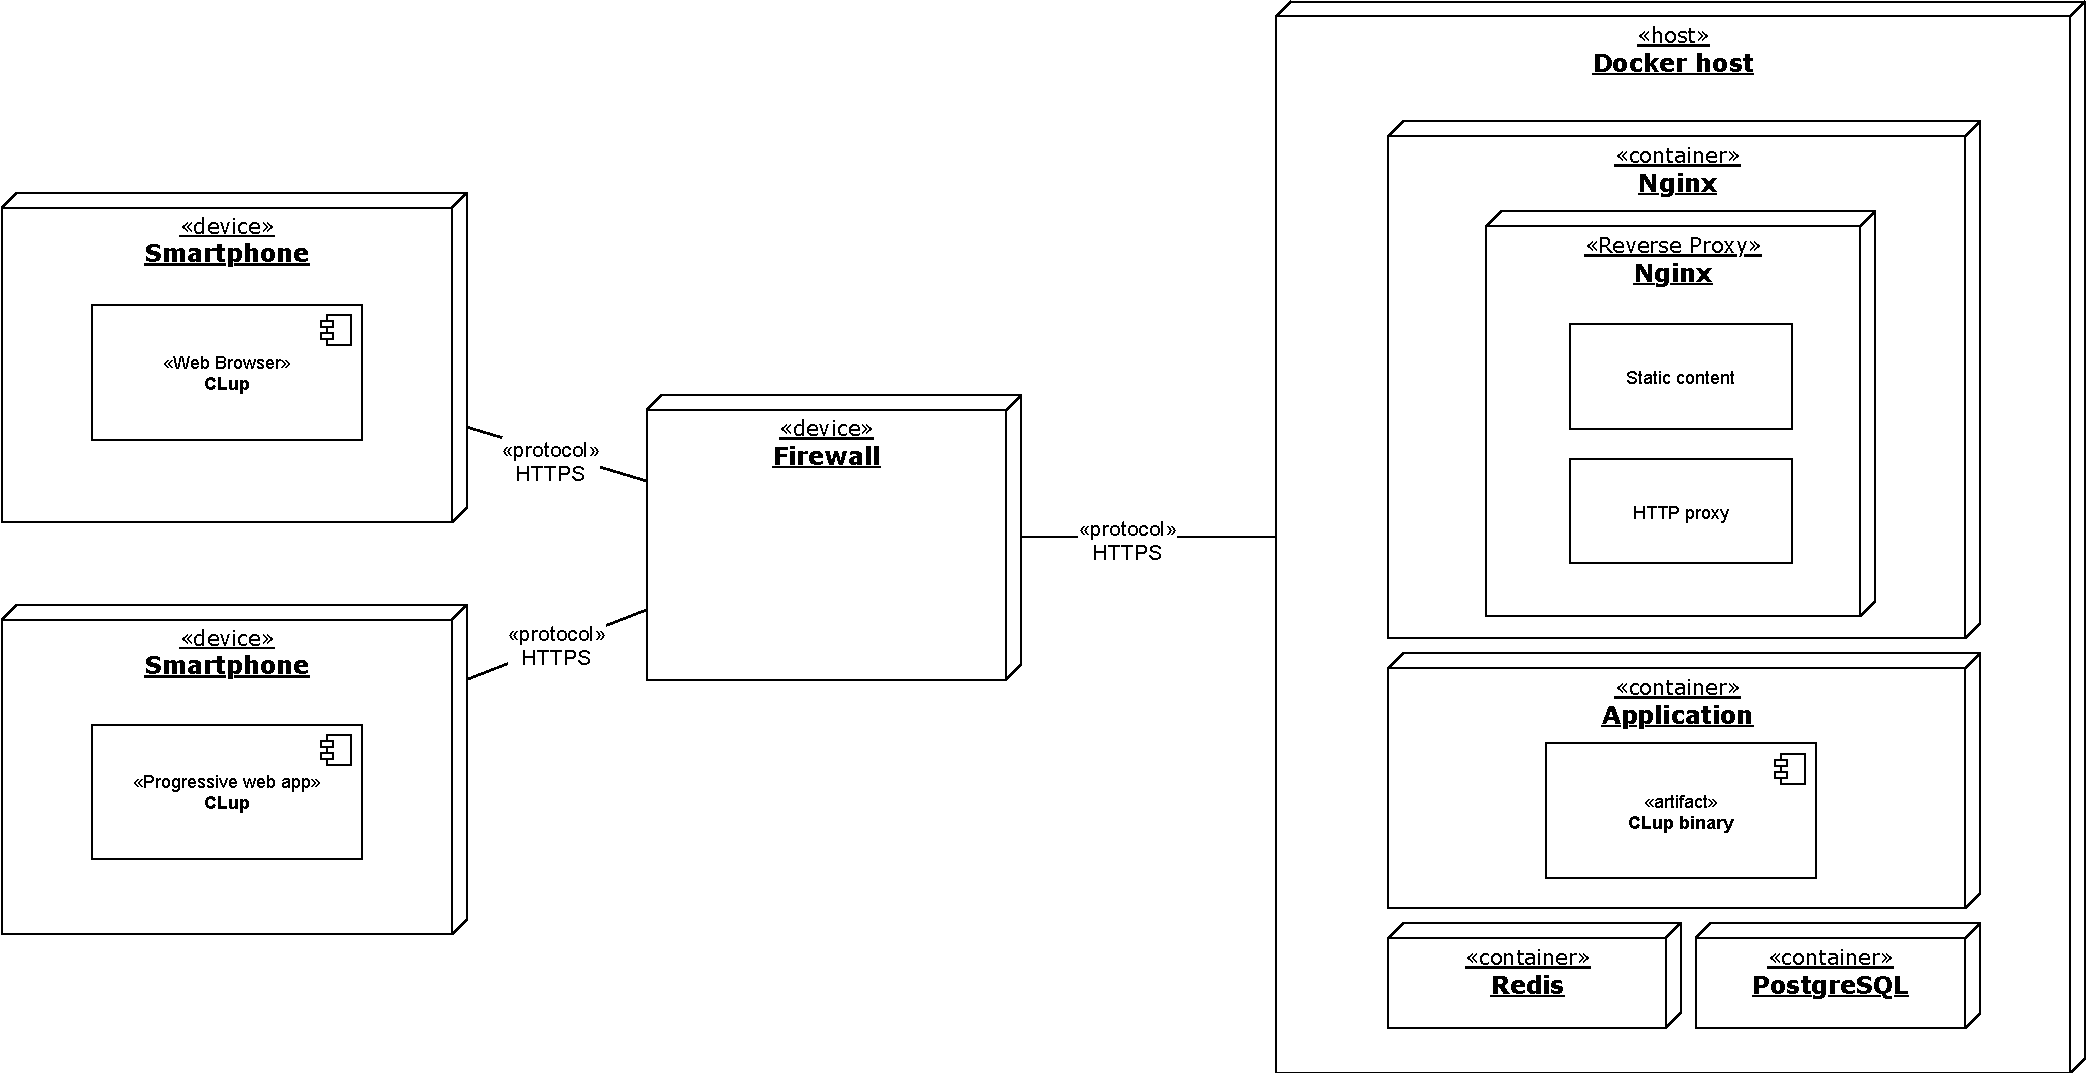
\includegraphics[width=1\textwidth]{Images/deployment-2.pdf}
    \caption{Deployment Diagram using Docker containers}
\end{figure}

The CLup application server should be deployable as separate artifacts for the components shown in Figure \ref{fig:component_diagram} to allow updating the services one at a time and limit service degradation in case of failures.

\subsection{Runtime view}
\begin{figure}[H]
    \centering
    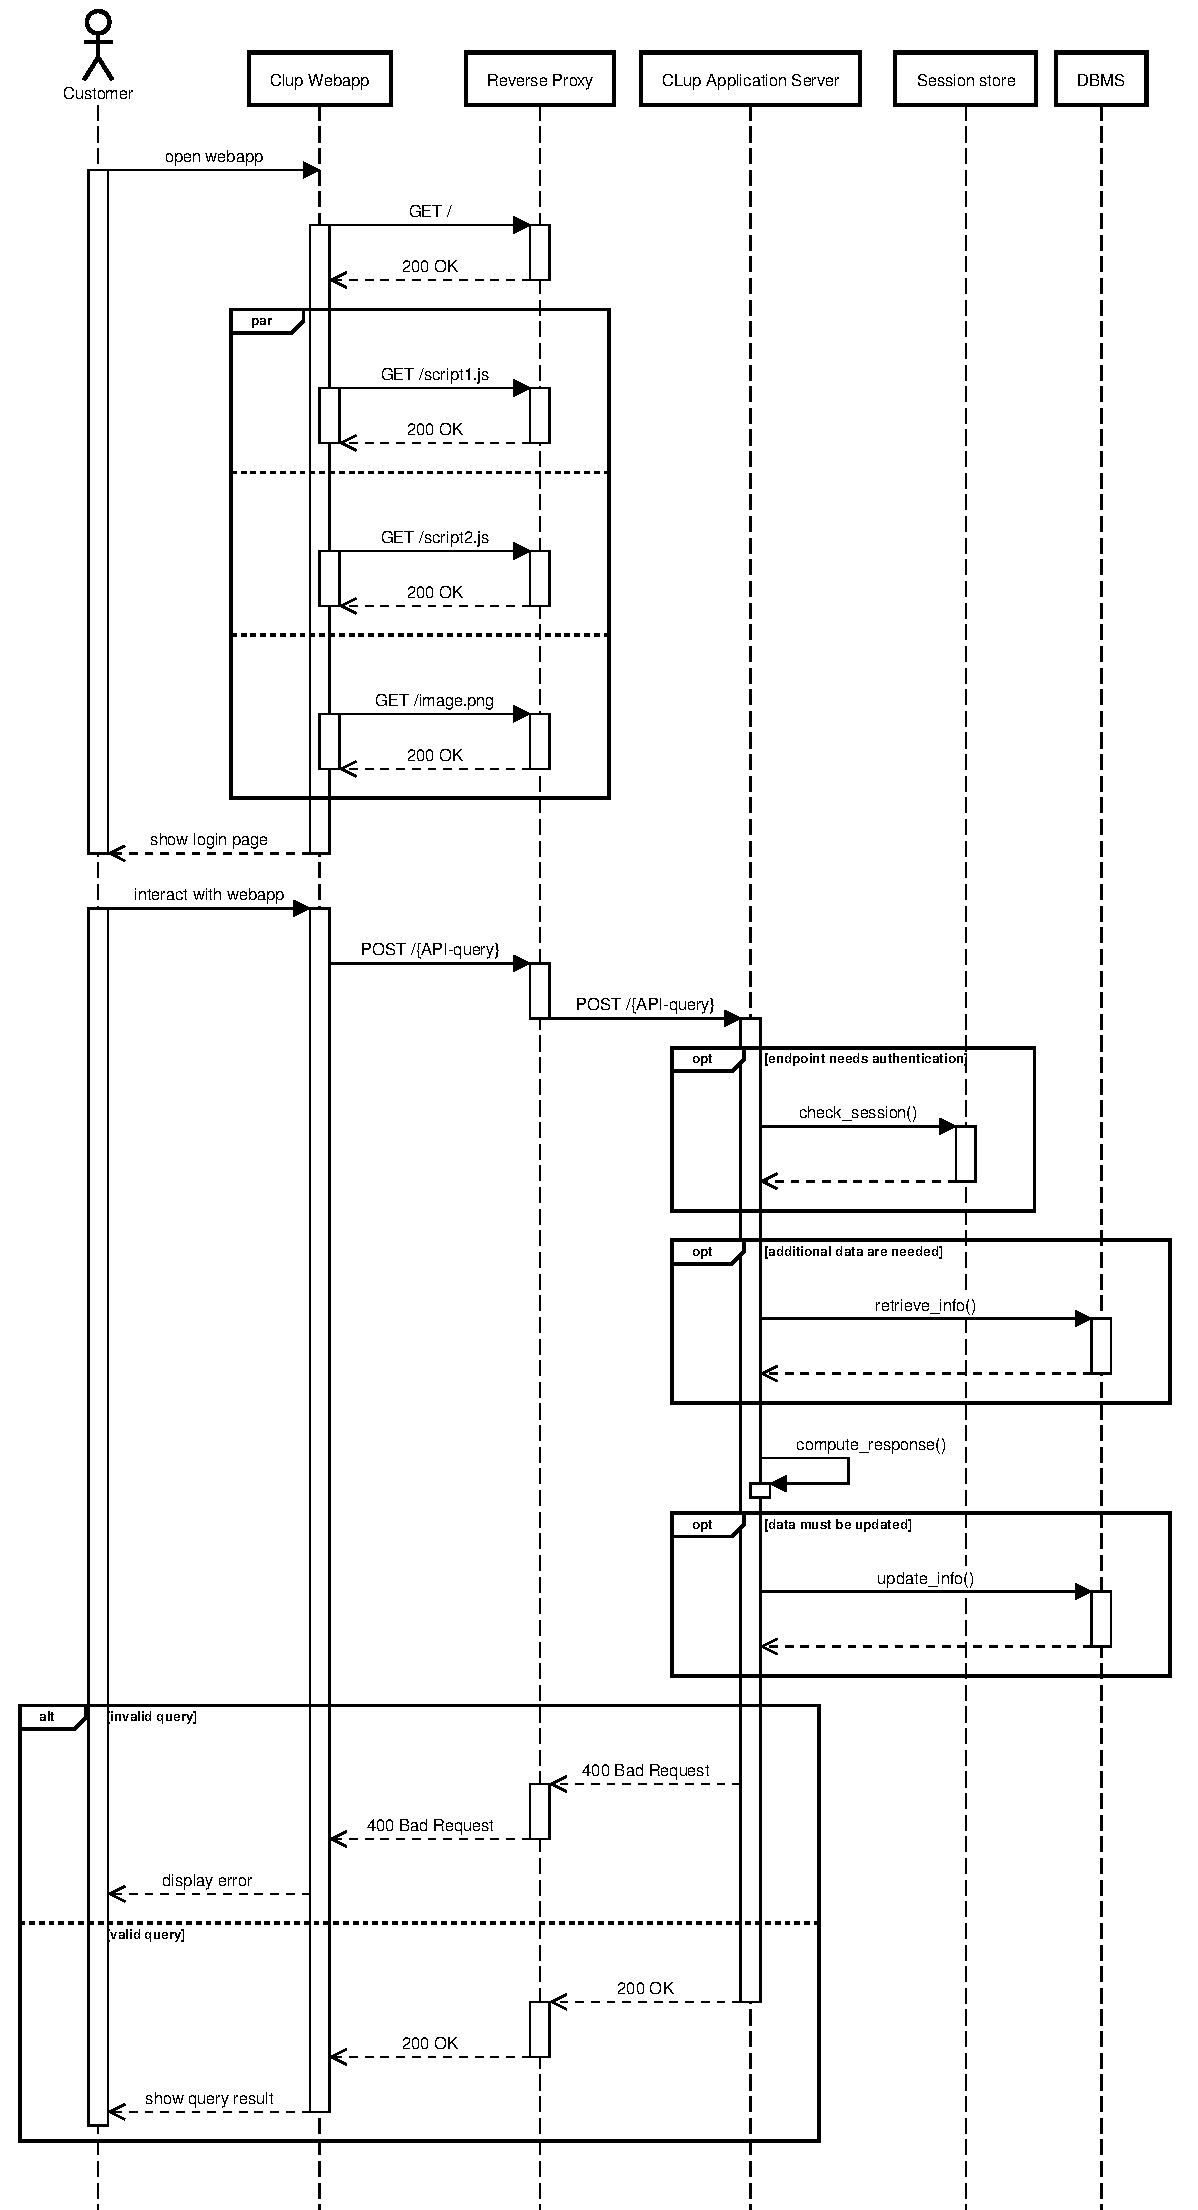
\includegraphics[height=0.9\textheight]{Images/runtime_revproxy.pdf}
    \caption{Generic API request (with detail of the Reverse Proxy)}
\end{figure}
\begin{figure}[H]
    \centering
    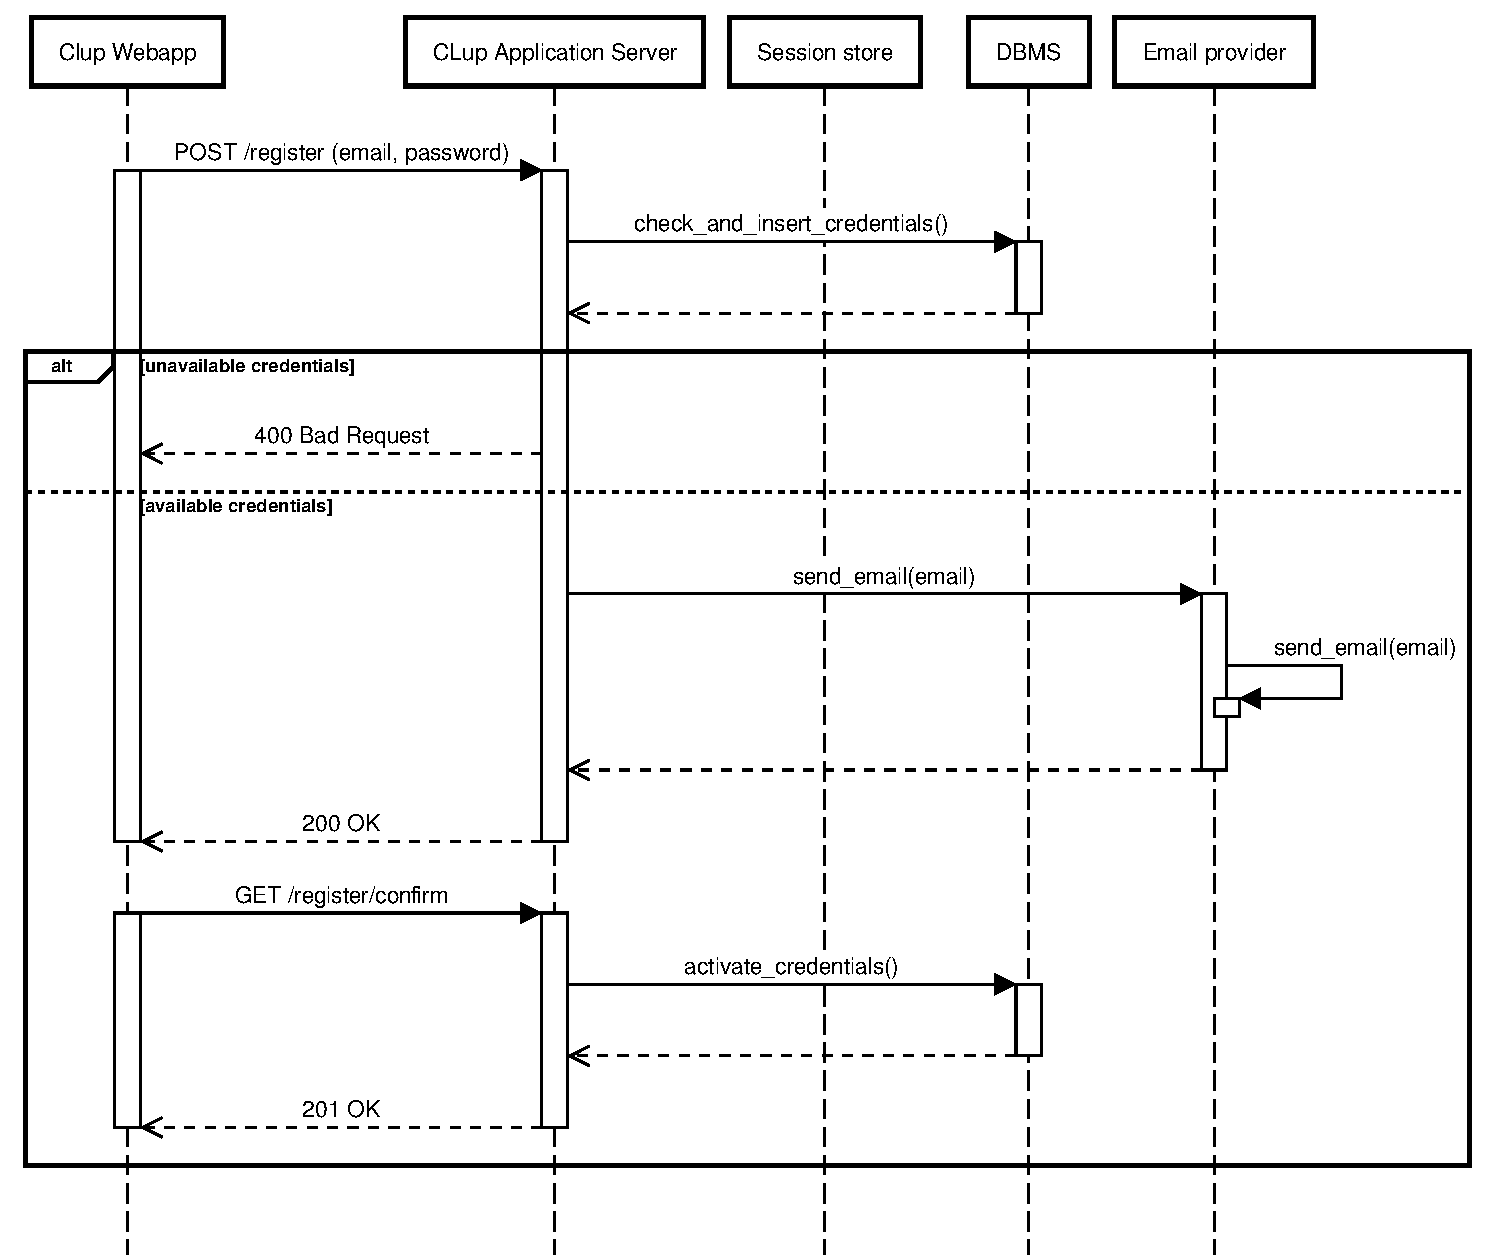
\includegraphics[width=1\textwidth]{Images/runtime_registration.pdf}
    \caption{Customer registering}
\end{figure}
\begin{figure}[H]
    \centering
    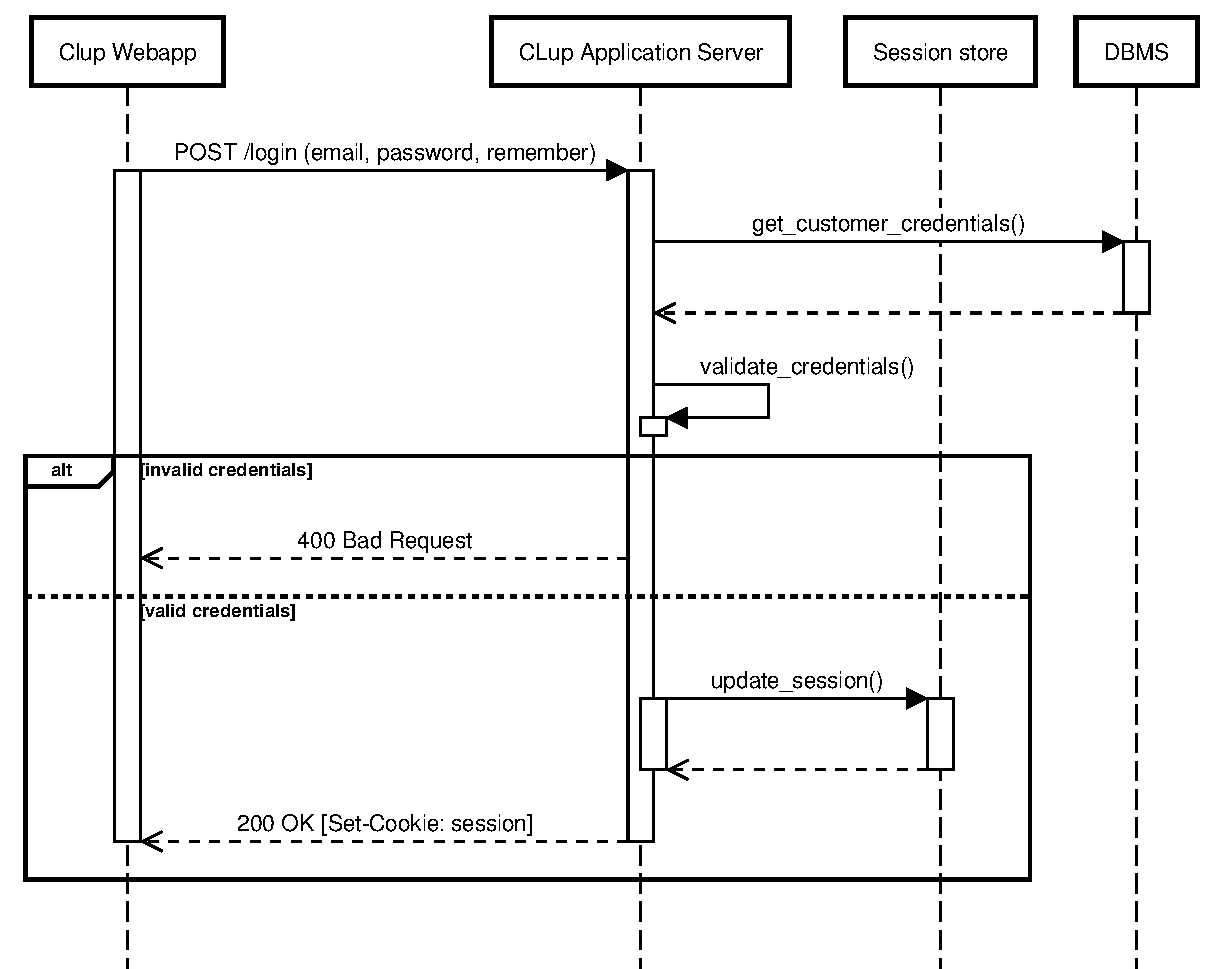
\includegraphics[width=1\textwidth]{Images/runtime_login.pdf}
    \caption{Customer logging in}
\end{figure}
\begin{figure}[H]
    \centering
    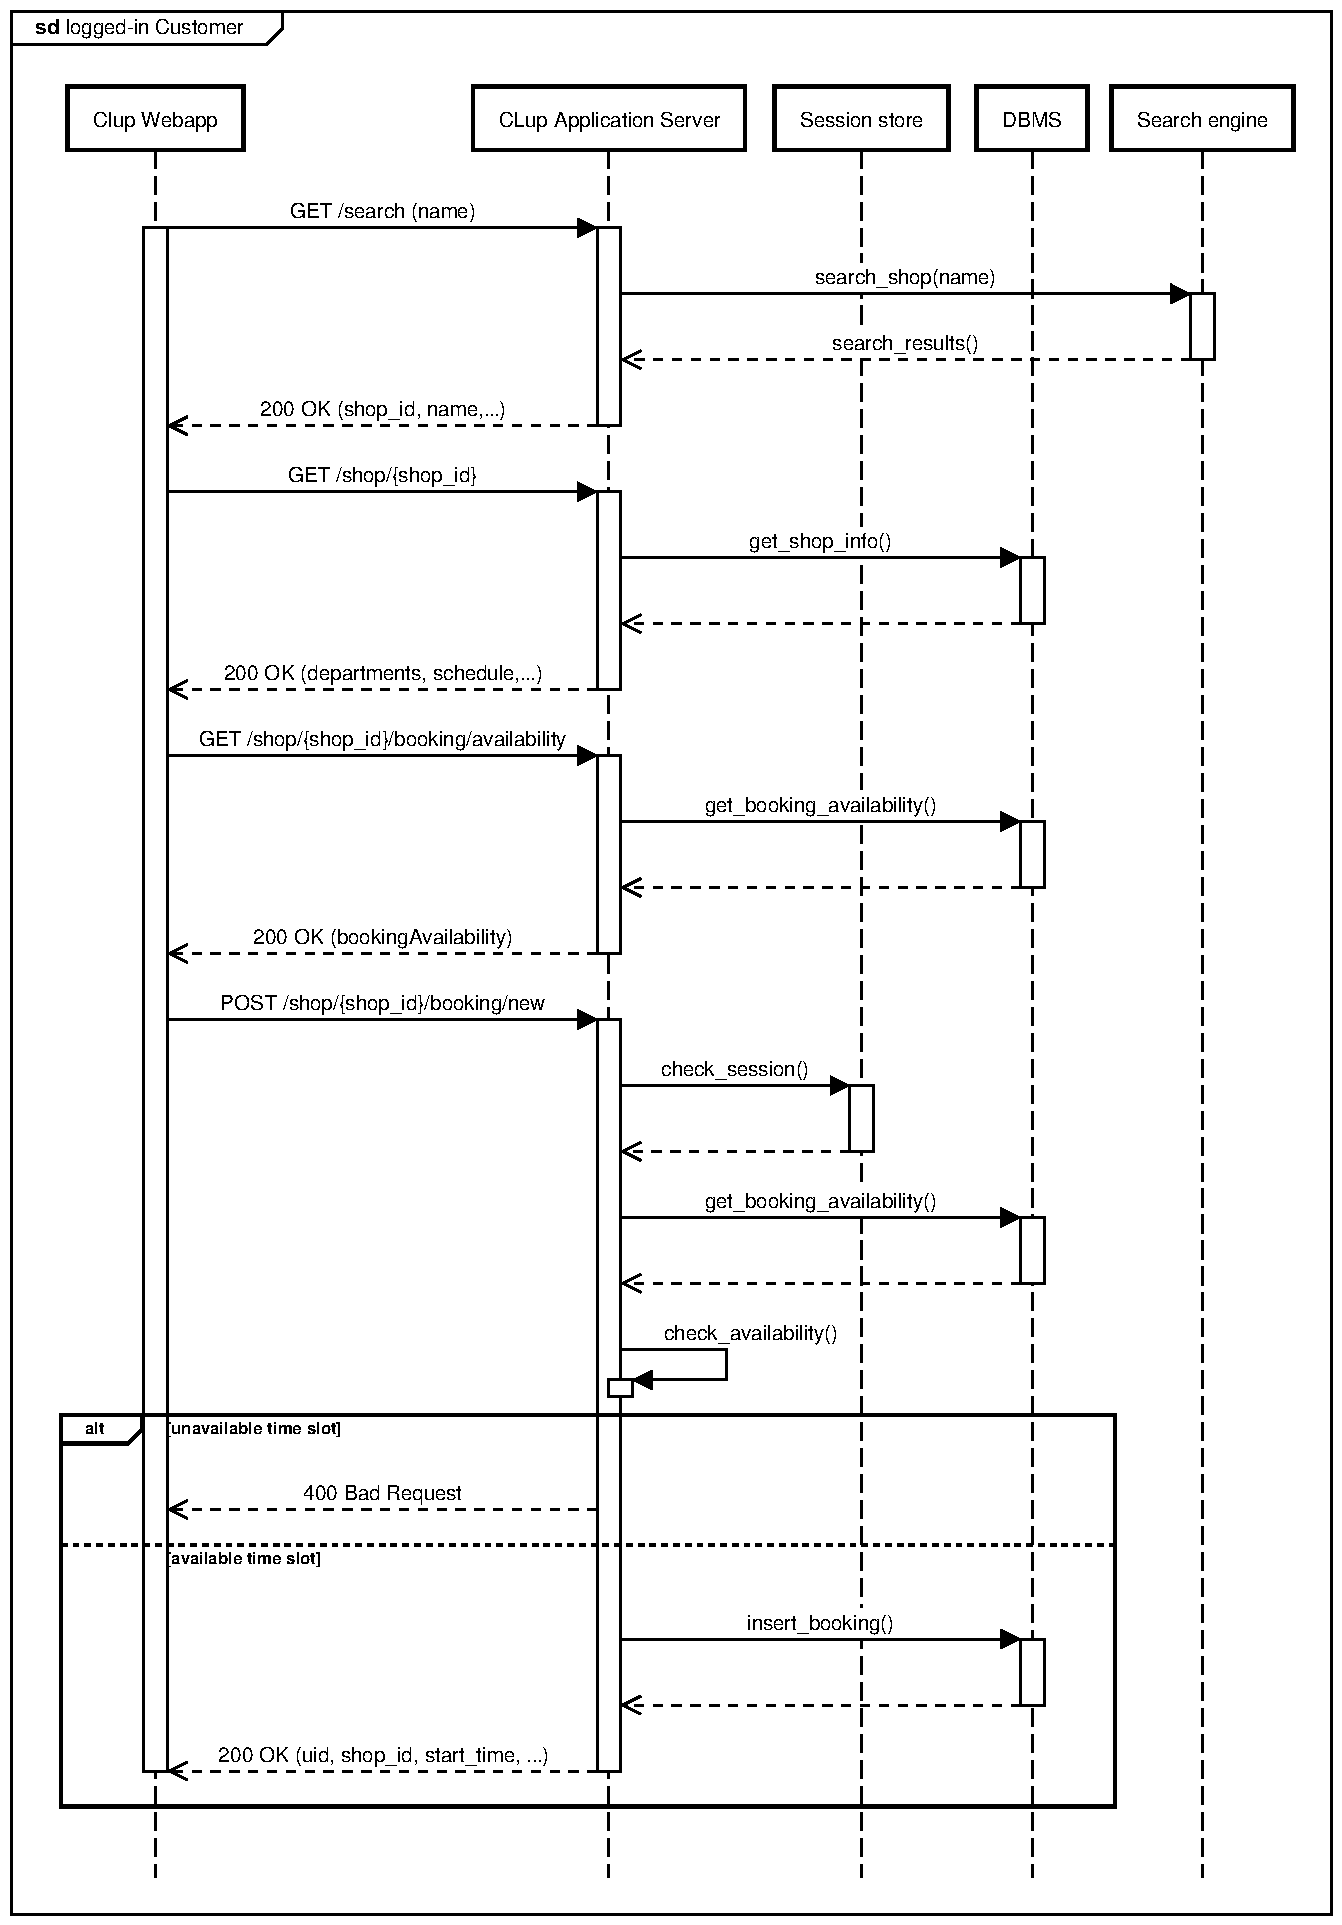
\includegraphics[width=1\textwidth]{Images/runtime_booking.pdf}
    \caption{Customer generating a Booking}
\end{figure}
\begin{figure}[H]
    \centering
    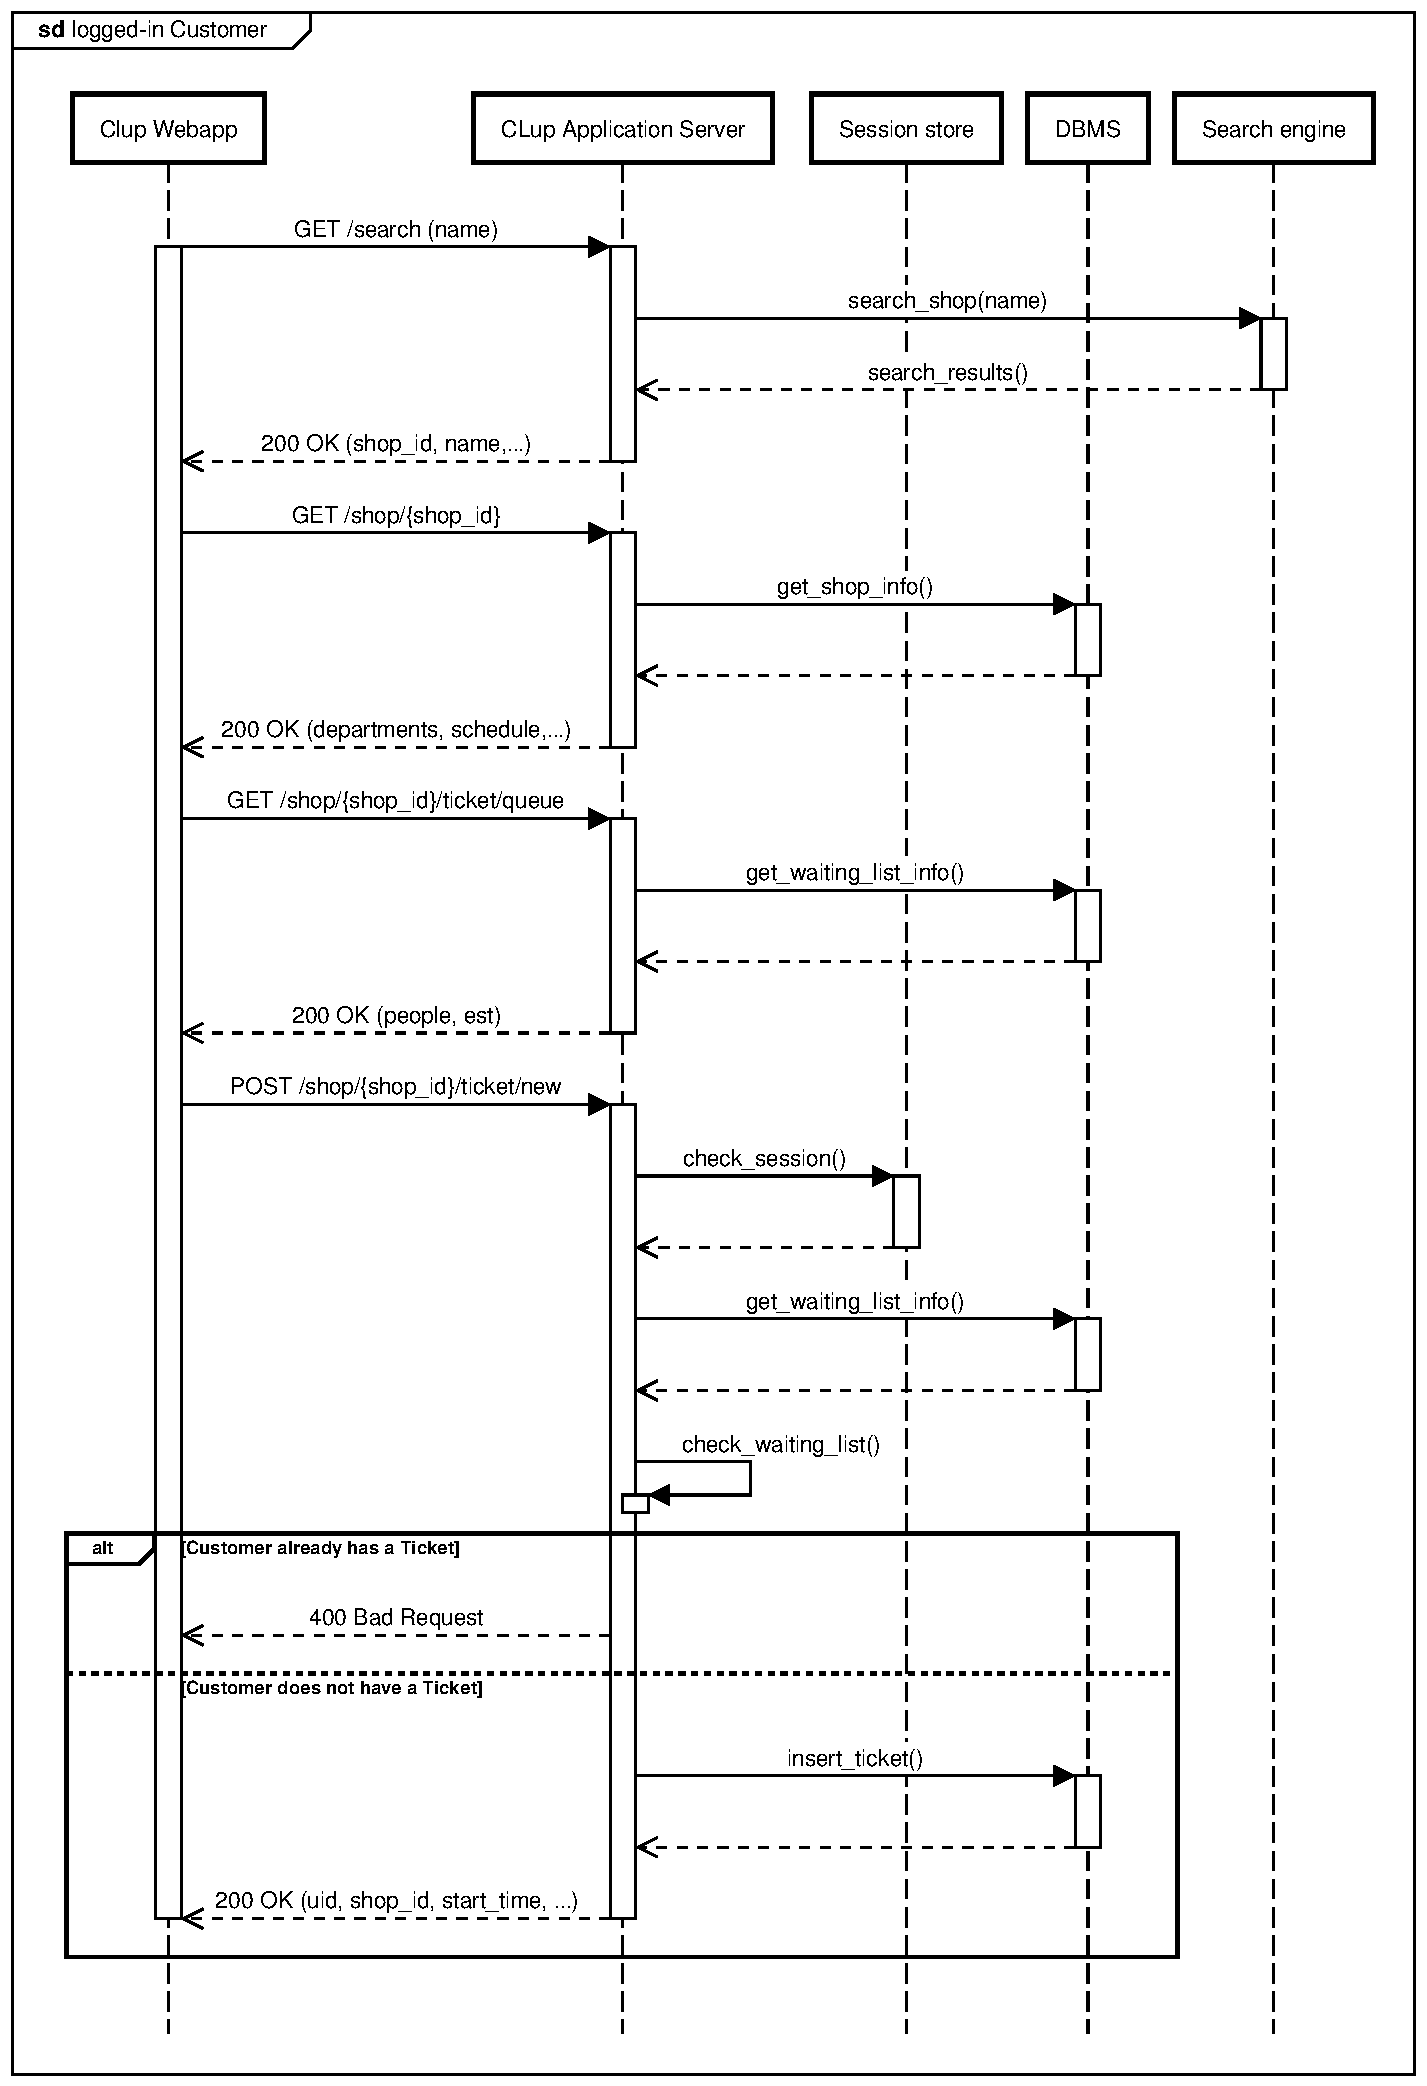
\includegraphics[width=1\textwidth]{Images/runtime_ticket.pdf}
    \caption{Customer generating a Ticket}
\end{figure}
\begin{figure}[H]
    \centering
    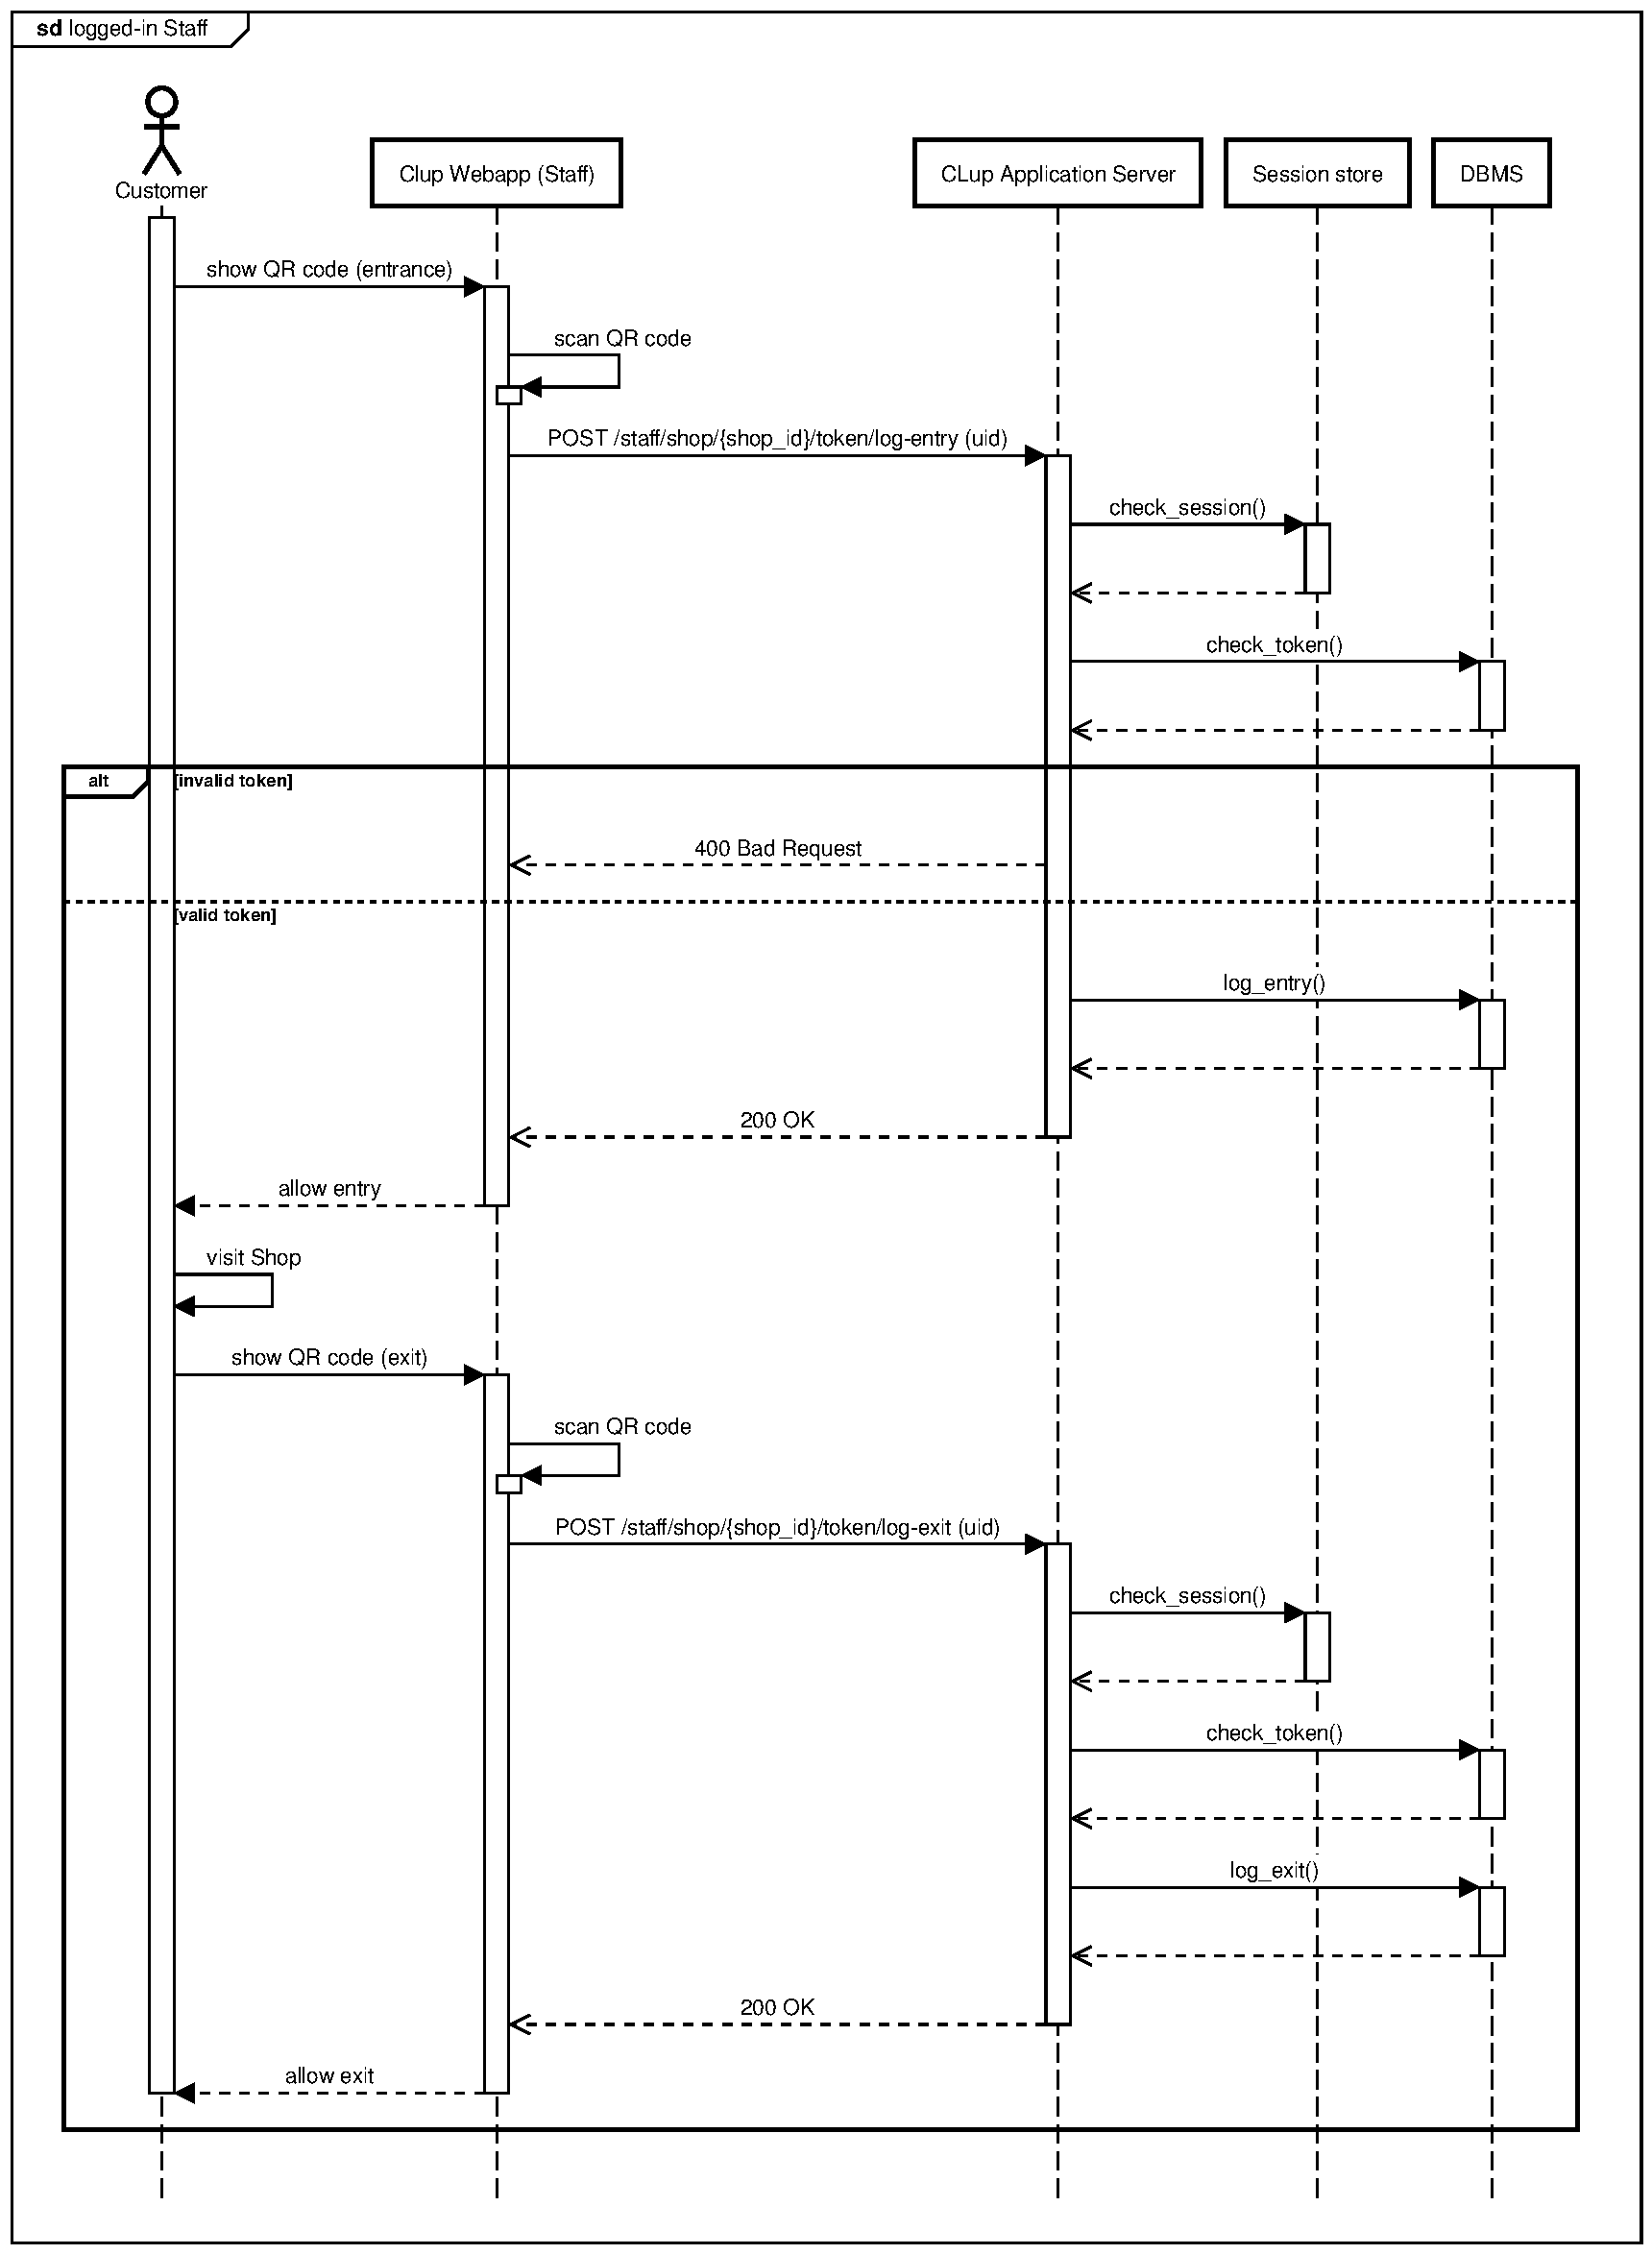
\includegraphics[width=1\textwidth]{Images/runtime_tokenvalidate.pdf}
    \caption{Staff validating either a Ticket or a Booking}
\end{figure}
\begin{figure}[H]
    \centering
    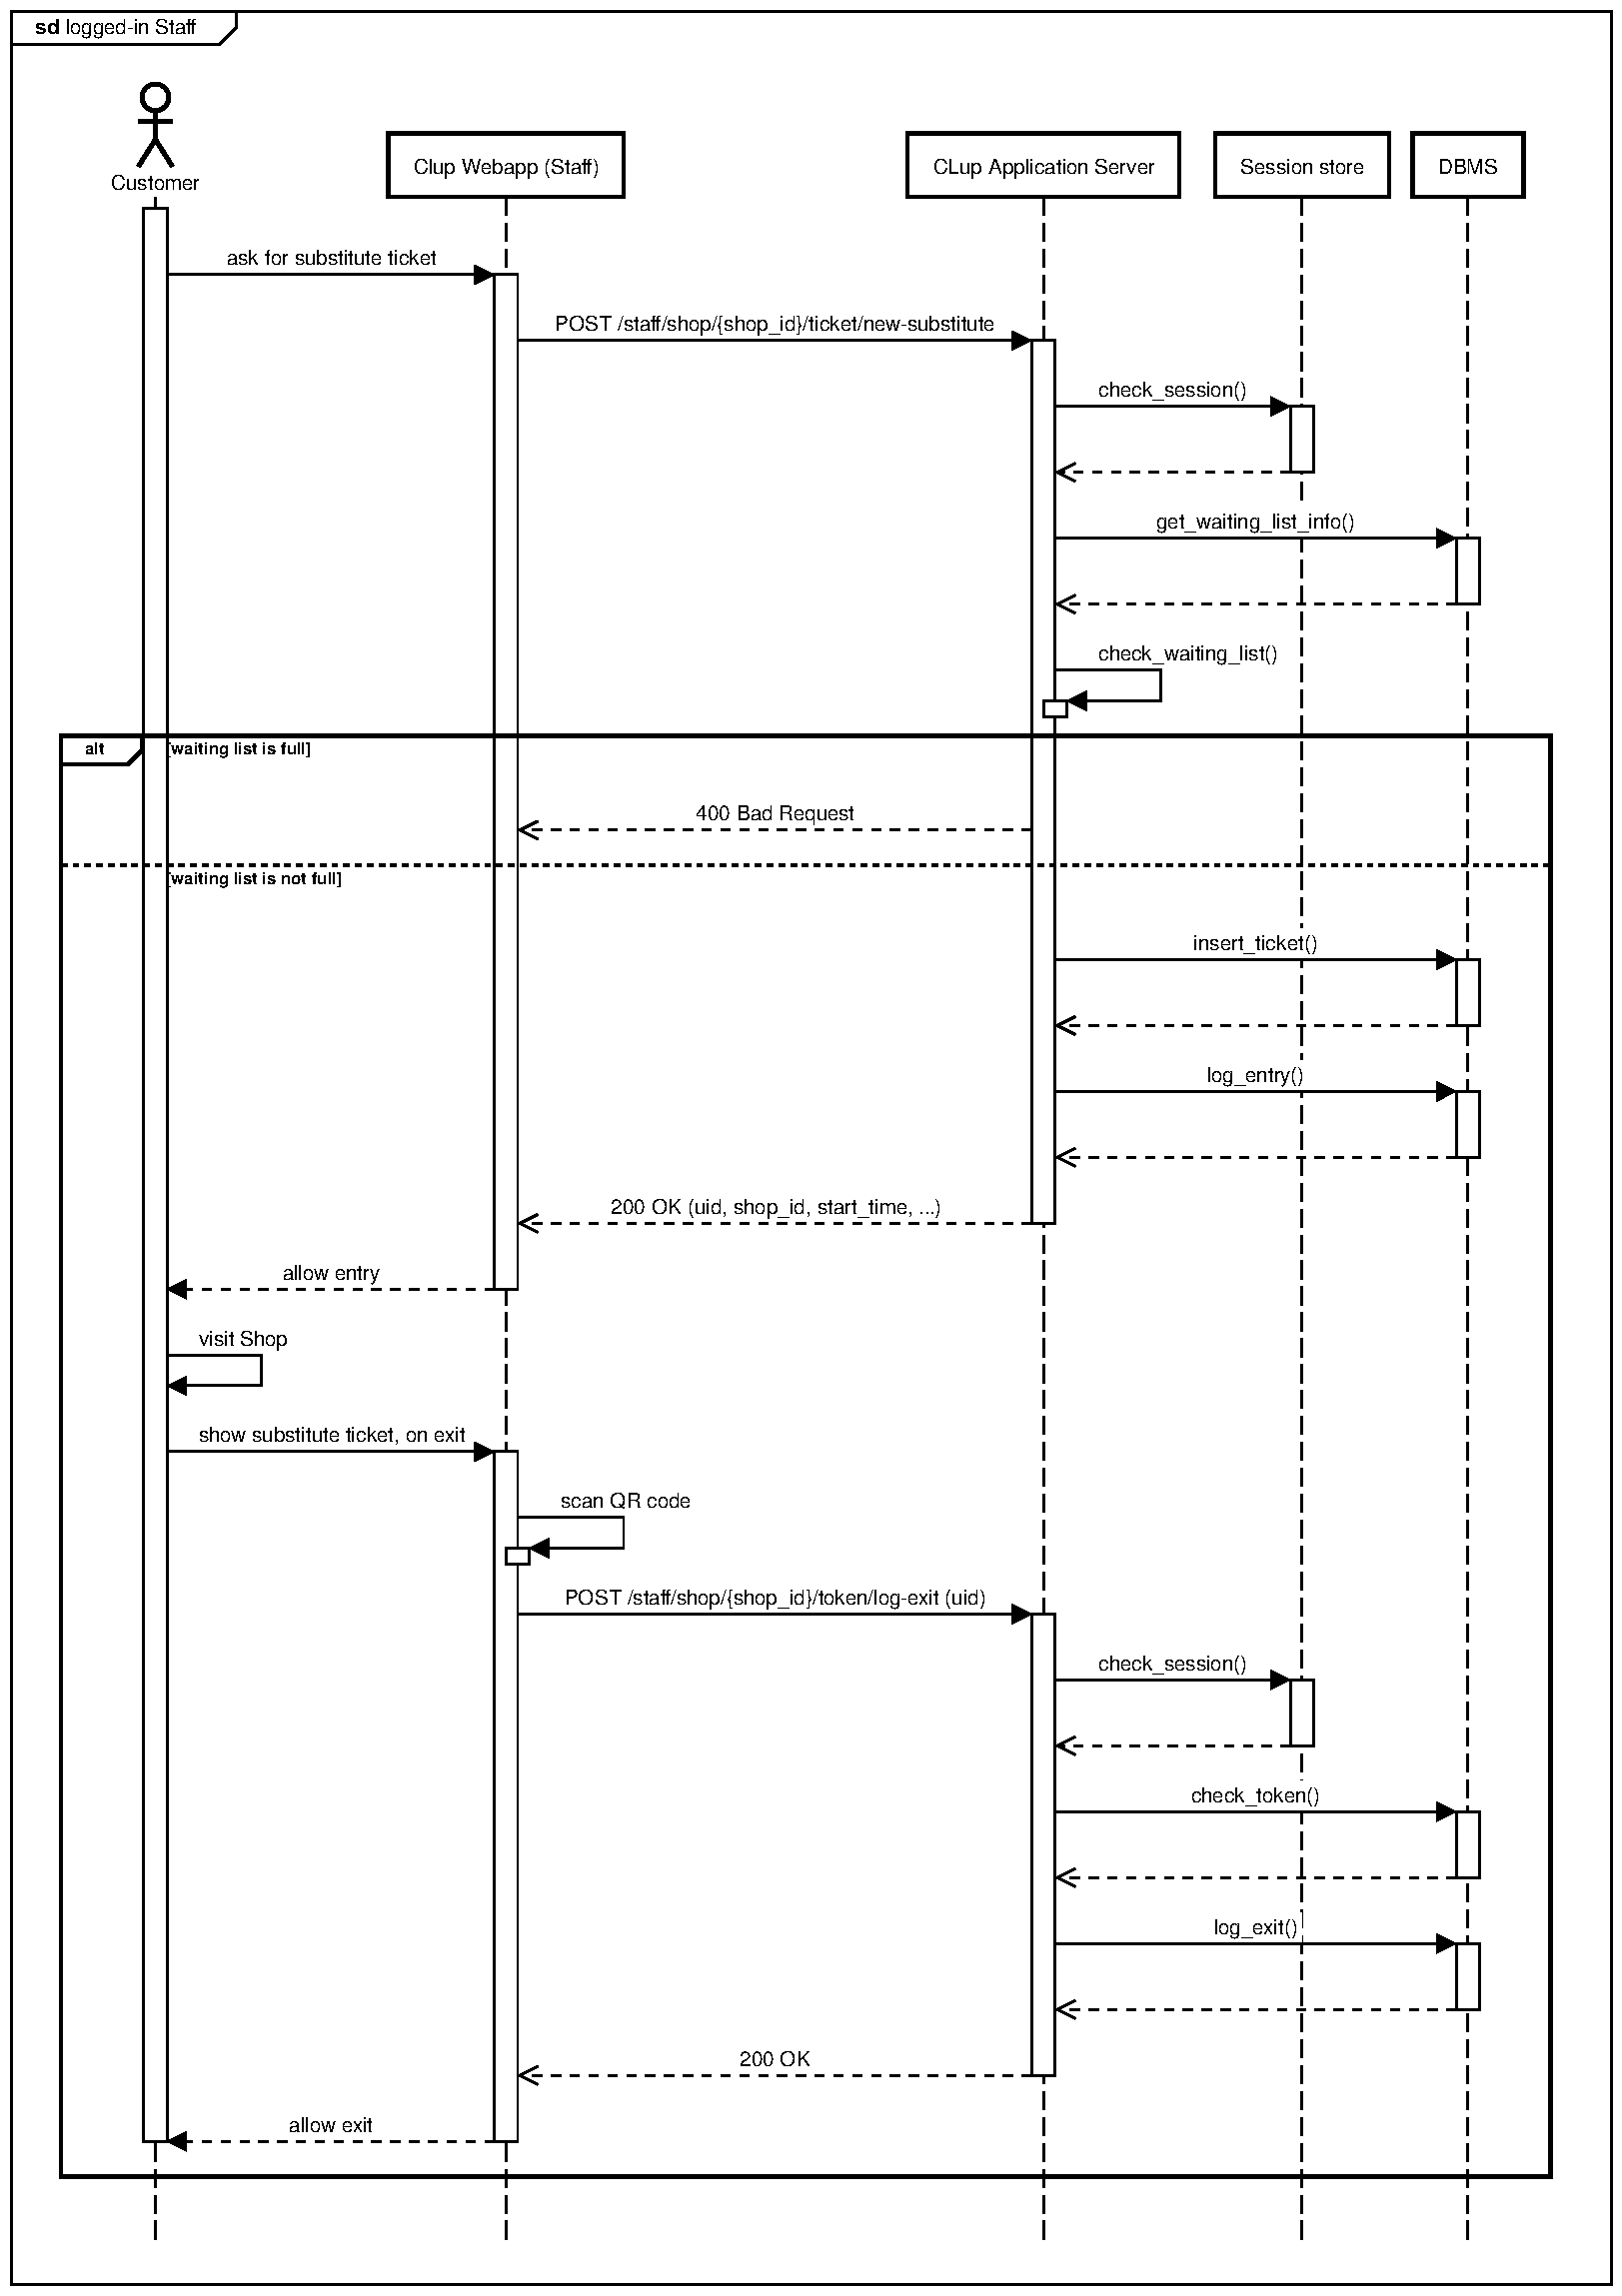
\includegraphics[width=1\textwidth]{Images/runtime_substitute.pdf}
    \caption{Staff generating a substitute Ticket}
\end{figure}

\subsection{Component interfaces}

\label{sect:api}
\subsubsection{API}


\begin{tabularx}{\textwidth}{|p{0.08\textwidth}|l|X|} \hline
\textbf{Class} & \textbf{HTTP request} & \textbf{Description} \\\hline\endhead
account & \makecell{\textbf{POST} \\ \texttt{/login}}  & Logs in and returns the authentication  cookie \\\hline
account & \makecell{\textbf{GET} \\ \texttt{/logout}}  & Log out and terminate session \\\hline
account & \makecell{\textbf{POST} \\ \texttt{/register}}  & Request creation of a new account \\\hline
account & \makecell{\textbf{GET} \\ \texttt{/register/confirm}}  & Submit email confirmation \\\hline
account & \makecell{\textbf{GET} \\ \texttt{/whoami}}  & Get customer authentication status \\\hline
booking & \makecell{\textbf{POST} \\ \texttt{/shop/\{shop\_id\}/booking/new}}  & Request a booking for a shop \\\hline
booking & \makecell{\textbf{GET} \\ \texttt{/shop/\{shop\_id\}/booking/availability}}  & Get information about the time slot availability for bookings \\\hline
manage & \makecell{\textbf{POST} \\ \texttt{/staff/manage/create-account/\{shop\_id\}}}  & Generate a temporary staff account for activation \\\hline
manage & \makecell{\textbf{POST} \\ \texttt{/staff/manage/shop/add}}  & Add a new shop to the database \\\hline
manage & \makecell{\textbf{POST} \\ \texttt{/staff/manage/shop/list}}  & Get a list of all managed shops \\\hline
manage & \makecell{\textbf{POST} \\ \texttt{/staff/manage/shop/\{shop\_id\}/edit}}  & Edit an existing shop listing \\\hline
manage & \makecell{\textbf{POST} \\ \texttt{/staff/manage/shop/\{shop\_id\}/show}}  & Make shop public and reachable from customers \\\hline
manage & \makecell{\textbf{POST} \\ \texttt{/staff/manage/shop/\{shop\_id\}/hide}}  & Make shop private and hidden from customers \\\hline
shop & \makecell{\textbf{GET} \\ \texttt{/search}}  & Search for a shop by name \\\hline
shop & \makecell{\textbf{GET} \\ \texttt{/shop/\{shop\_id\}}}  & Get available shop information \\\hline
staff & \makecell{\textbf{GET} \\ \texttt{/staff/shop/\{shop\_id\}/ticket/queue}}  & Get detailed information about the current queue status \\\hline
staff & \makecell{\textbf{GET} \\ \texttt{/staff/shop/\{shop\_id\}/booking/list}}  & Get detailed information about the current and future bookings \\\hline
staff & \makecell{\textbf{GET} \\ \texttt{/staff/shop/\{shop\_id\}/token/info}}  & Get token information and validity \\\hline
staff & \makecell{\textbf{GET} \\ \texttt{/staff/shop/\{shop\_id\}/status}}  & Get token information and validity \\\hline
staff & \makecell{\textbf{POST} \\ \texttt{/staff/shop/\{shop\_id\}/ticket/new-substitute}}  & Request creation of a substitute ticket \\\hline
staff & \makecell{\textbf{POST} \\ \texttt{/staff/shop/\{shop\_id\}/token/log-entry}}  & Log entry, consume the token and update shop occupancy information \\\hline
staff & \makecell{\textbf{POST} \\ \texttt{/staff/shop/\{shop\_id\}/token/log-exit}}  & Log exit, update shop occupancy information \\\hline
staff-account & \makecell{\textbf{POST} \\ \texttt{/staff/login}}  & Log in and return authentication cookie \\\hline
staff-account & \makecell{\textbf{POST} \\ \texttt{/staff/register}}  & Activate staff account and set password \\\hline
ticket & \makecell{\textbf{GET} \\ \texttt{/ticket/est}}  & Get the estimated waiting time for a ticket \\\hline
ticket & \makecell{\textbf{POST} \\ \texttt{/shop/\{shop\_id\}/ticket/new}}  & Request a ticket for a shop \\\hline
ticket & \makecell{\textbf{POST} \\ \texttt{/ticket/cancel}}  & Cancel a ticket \\\hline
ticket & \makecell{\textbf{GET} \\ \texttt{/shop/\{shop\_id\}/ticket/queue}}  & Get information about the queue status and approximate waiting time \\\hline
token & \makecell{\textbf{GET} \\ \texttt{/tokens}}  & Get active tokens for the customer \\\hline
\end{tabularx}

\subsubsection{Endpoints}

\begin{table}[H]
\tabulinesep=4pt\everyrow{\tabucline[0.5pt]-}
\begin{tabu} to \textwidth {@{}|X|X[5]|} \hline
\textbf{POST}  & \texttt{/login} \\
Description   & Logs in and returns the authentication  cookie  \\
Body & \texttt{RequestLogin} \\
Responses     & \everyrow{}\begin{tabu}{X[0.5]|X[3]|X[2]} 
\textbf{Code} & \textbf{Description} & \textbf{Body} \\
\hline \textbf{200} & OK &\\
\hline \textbf{400} & Invalid Credentials &\\
\end{tabu}\everyrow{\tabucline[0.5pt]-} \\
\end{tabu}
\end{table}
\begin{table}[H]
\tabulinesep=4pt\everyrow{\tabucline[0.5pt]-}
\begin{tabu} to \textwidth {@{}|X|X[5]|} \hline
\textbf{GET}  & \texttt{/logout} \\
Description   & Log out and terminate session  \\
Responses     & \everyrow{}\begin{tabu}{X[0.5]|X[3]|X[2]} 
\textbf{Code} & \textbf{Description} & \textbf{Body} \\
\hline \textbf{200} & OK &\\
\hline \textbf{400} & Not Logged in &\\
\end{tabu}\everyrow{\tabucline[0.5pt]-} \\
\end{tabu}
\end{table}
\begin{table}[H]
\tabulinesep=4pt\everyrow{\tabucline[0.5pt]-}
\begin{tabu} to \textwidth {@{}|X|X[5]|} \hline
\textbf{POST}  & \texttt{/register} \\
Description   & Request creation of a new account  \\
Body & \texttt{RequestRegistration} \\
Responses     & \everyrow{}\begin{tabu}{X[0.5]|X[3]|X[2]} 
\textbf{Code} & \textbf{Description} & \textbf{Body} \\
\hline \textbf{200} & OK &\\
\hline \textbf{400} & Invalid data &\\
\end{tabu}\everyrow{\tabucline[0.5pt]-} \\
\end{tabu}
\end{table}
\begin{table}[H]
\tabulinesep=4pt\everyrow{\tabucline[0.5pt]-}
\begin{tabu} to \textwidth {@{}|X|X[5]|} \hline
\textbf{GET}  & \texttt{/register/confirm} \\
Description   & Submit email confirmation  \\
Parameters    & \everyrow{}\begin{tabu}{X|X}
\textbf{Name} & \textbf{Type} \\
\hline code & \texttt{string} \\
\end{tabu}\everyrow{\tabucline[0.5pt]-}\\
Responses     & \everyrow{}\begin{tabu}{X[0.5]|X[3]|X[2]} 
\textbf{Code} & \textbf{Description} & \textbf{Body} \\
\hline \textbf{201} & successful operation &\\
\hline \textbf{400} & Invalid code &\\
\end{tabu}\everyrow{\tabucline[0.5pt]-} \\
\end{tabu}
\end{table}
\begin{table}[H]
\tabulinesep=4pt\everyrow{\tabucline[0.5pt]-}
\begin{tabu} to \textwidth {@{}|X|X[5]|} \hline
\textbf{GET}  & \texttt{/whoami} \\
Description   & Get customer authentication status  \\
Responses     & \everyrow{}\begin{tabu}{X[0.5]|X[3]|X[2]} 
\textbf{Code} & \textbf{Description} & \textbf{Body} \\
\hline \textbf{200} & Ok &\texttt{\{authenticated: boolean, email: string,\}}\\
\end{tabu}\everyrow{\tabucline[0.5pt]-} \\
\end{tabu}
\end{table}
\begin{table}[H]
\tabulinesep=4pt\everyrow{\tabucline[0.5pt]-}
\begin{tabu} to \textwidth {@{}|X|X[5]|} \hline
\textbf{POST}  & \texttt{/shop/\{shop\_id\}/booking/new} \\
Description   & Request a booking for a shop  \\
Parameters    & \everyrow{}\begin{tabu}{X|X}
\textbf{Name} & \textbf{Type} \\
\hline shop\_id & \texttt{string} \\
\end{tabu}\everyrow{\tabucline[0.5pt]-}\\
Body & \texttt{RequestBooking} \\
Responses     & \everyrow{}\begin{tabu}{X[0.5]|X[3]|X[2]} 
\textbf{Code} & \textbf{Description} & \textbf{Body} \\
\hline \textbf{200} & OK &\texttt{TokenBooking}\\
\hline \textbf{400} & Error &\\
\end{tabu}\everyrow{\tabucline[0.5pt]-} \\
\end{tabu}
\end{table}
\begin{table}[H]
\tabulinesep=4pt\everyrow{\tabucline[0.5pt]-}
\begin{tabu} to \textwidth {@{}|X|X[5]|} \hline
\textbf{GET}  & \texttt{/shop/\{shop\_id\}/booking/availability} \\
Description   & Get information about the time slot availability for bookings  \\
Parameters    & \everyrow{}\begin{tabu}{X|X}
\textbf{Name} & \textbf{Type} \\
\hline shop\_id & \texttt{string} \\
\hline day & \texttt{string} \\
\end{tabu}\everyrow{\tabucline[0.5pt]-}\\
Responses     & \everyrow{}\begin{tabu}{X[0.5]|X[3]|X[2]} 
\textbf{Code} & \textbf{Description} & \textbf{Body} \\
\hline \textbf{200} & OK &\texttt{BookingAvailability}\\
\hline \textbf{400} & Error &\\
\end{tabu}\everyrow{\tabucline[0.5pt]-} \\
\end{tabu}
\end{table}
\begin{table}[H]
\tabulinesep=4pt\everyrow{\tabucline[0.5pt]-}
\begin{tabu} to \textwidth {@{}|X|X[5]|} \hline
\textbf{POST}  & \texttt{/staff/manage/create-account/\{shop\_id\}} \\
Description   & Generate a temporary staff account for activation  \\
Parameters    & \everyrow{}\begin{tabu}{X|X}
\textbf{Name} & \textbf{Type} \\
\hline shop\_id & \texttt{string} \\
\end{tabu}\everyrow{\tabucline[0.5pt]-}\\
Body & \texttt{string} \\
Responses     & \everyrow{}\begin{tabu}{X[0.5]|X[3]|X[2]} 
\textbf{Code} & \textbf{Description} & \textbf{Body} \\
\hline \textbf{200} & OK &\texttt{StaffTempAccount}\\
\hline \textbf{400} & Invalid email &\\
\end{tabu}\everyrow{\tabucline[0.5pt]-} \\
\end{tabu}
\end{table}
\begin{table}[H]
\tabulinesep=4pt\everyrow{\tabucline[0.5pt]-}
\begin{tabu} to \textwidth {@{}|X|X[5]|} \hline
\textbf{POST}  & \texttt{/staff/manage/shop/add} \\
Description   & Add a new shop to the database  \\
Body & \texttt{string} \\
Responses     & \everyrow{}\begin{tabu}{X[0.5]|X[3]|X[2]} 
\textbf{Code} & \textbf{Description} & \textbf{Body} \\
\hline \textbf{200} & OK &\texttt{Shop}\\
\end{tabu}\everyrow{\tabucline[0.5pt]-} \\
\end{tabu}
\end{table}
\begin{table}[H]
\tabulinesep=4pt\everyrow{\tabucline[0.5pt]-}
\begin{tabu} to \textwidth {@{}|X|X[5]|} \hline
\textbf{POST}  & \texttt{/staff/manage/shop/list} \\
Description   & Get a list of all managed shops  \\
Responses     & \everyrow{}\begin{tabu}{X[0.5]|X[3]|X[2]} 
\textbf{Code} & \textbf{Description} & \textbf{Body} \\
\hline \textbf{200} & OK &\texttt{Array<SearchResult>}\\
\end{tabu}\everyrow{\tabucline[0.5pt]-} \\
\end{tabu}
\end{table}
\begin{table}[H]
\tabulinesep=4pt\everyrow{\tabucline[0.5pt]-}
\begin{tabu} to \textwidth {@{}|X|X[5]|} \hline
\textbf{POST}  & \texttt{/staff/manage/shop/\{shop\_id\}/edit} \\
Description   & Edit an existing shop listing  \\
Parameters    & \everyrow{}\begin{tabu}{X|X}
\textbf{Name} & \textbf{Type} \\
\hline shop\_id & \texttt{string} \\
\end{tabu}\everyrow{\tabucline[0.5pt]-}\\
Body & \texttt{Shop} \\
Responses     & \everyrow{}\begin{tabu}{X[0.5]|X[3]|X[2]} 
\textbf{Code} & \textbf{Description} & \textbf{Body} \\
\hline \textbf{200} & OK &\\
\end{tabu}\everyrow{\tabucline[0.5pt]-} \\
\end{tabu}
\end{table}
\begin{table}[H]
\tabulinesep=4pt\everyrow{\tabucline[0.5pt]-}
\begin{tabu} to \textwidth {@{}|X|X[5]|} \hline
\textbf{POST}  & \texttt{/staff/manage/shop/\{shop\_id\}/show} \\
Description   & Make shop public and reachable from customers  \\
Parameters    & \everyrow{}\begin{tabu}{X|X}
\textbf{Name} & \textbf{Type} \\
\hline shop\_id & \texttt{string} \\
\end{tabu}\everyrow{\tabucline[0.5pt]-}\\
Responses     & \everyrow{}\begin{tabu}{X[0.5]|X[3]|X[2]} 
\textbf{Code} & \textbf{Description} & \textbf{Body} \\
\hline \textbf{200} & OK &\\
\end{tabu}\everyrow{\tabucline[0.5pt]-} \\
\end{tabu}
\end{table}
\begin{table}[H]
\tabulinesep=4pt\everyrow{\tabucline[0.5pt]-}
\begin{tabu} to \textwidth {@{}|X|X[5]|} \hline
\textbf{POST}  & \texttt{/staff/manage/shop/\{shop\_id\}/hide} \\
Description   & Make shop private and hidden from customers  \\
Parameters    & \everyrow{}\begin{tabu}{X|X}
\textbf{Name} & \textbf{Type} \\
\hline shop\_id & \texttt{string} \\
\end{tabu}\everyrow{\tabucline[0.5pt]-}\\
Responses     & \everyrow{}\begin{tabu}{X[0.5]|X[3]|X[2]} 
\textbf{Code} & \textbf{Description} & \textbf{Body} \\
\hline \textbf{200} & OK &\\
\end{tabu}\everyrow{\tabucline[0.5pt]-} \\
\end{tabu}
\end{table}
\begin{table}[H]
\tabulinesep=4pt\everyrow{\tabucline[0.5pt]-}
\begin{tabu} to \textwidth {@{}|X|X[5]|} \hline
\textbf{GET}  & \texttt{/search} \\
Description   & Search for a shop by name  \\
Parameters    & \everyrow{}\begin{tabu}{X|X}
\textbf{Name} & \textbf{Type} \\
\hline q & \texttt{string} \\
\end{tabu}\everyrow{\tabucline[0.5pt]-}\\
Responses     & \everyrow{}\begin{tabu}{X[0.5]|X[3]|X[2]} 
\textbf{Code} & \textbf{Description} & \textbf{Body} \\
\hline \textbf{200} & OK &\texttt{Array<SearchResult>}\\
\end{tabu}\everyrow{\tabucline[0.5pt]-} \\
\end{tabu}
\end{table}
\begin{table}[H]
\tabulinesep=4pt\everyrow{\tabucline[0.5pt]-}
\begin{tabu} to \textwidth {@{}|X|X[5]|} \hline
\textbf{GET}  & \texttt{/shop/\{shop\_id\}} \\
Description   & Get available shop information  \\
Parameters    & \everyrow{}\begin{tabu}{X|X}
\textbf{Name} & \textbf{Type} \\
\hline shop\_id & \texttt{string} \\
\end{tabu}\everyrow{\tabucline[0.5pt]-}\\
Responses     & \everyrow{}\begin{tabu}{X[0.5]|X[3]|X[2]} 
\textbf{Code} & \textbf{Description} & \textbf{Body} \\
\hline \textbf{200} & OK &\texttt{Shop}\\
\end{tabu}\everyrow{\tabucline[0.5pt]-} \\
\end{tabu}
\end{table}
\begin{table}[H]
\tabulinesep=4pt\everyrow{\tabucline[0.5pt]-}
\begin{tabu} to \textwidth {@{}|X|X[5]|} \hline
\textbf{GET}  & \texttt{/staff/shop/\{shop\_id\}/ticket/queue} \\
Description   & Get detailed information about the current queue status  \\
Parameters    & \everyrow{}\begin{tabu}{X|X}
\textbf{Name} & \textbf{Type} \\
\hline shop\_id & \texttt{string} \\
\end{tabu}\everyrow{\tabucline[0.5pt]-}\\
Responses     & \everyrow{}\begin{tabu}{X[0.5]|X[3]|X[2]} 
\textbf{Code} & \textbf{Description} & \textbf{Body} \\
\hline \textbf{200} & OK &\texttt{Queue}\\
\end{tabu}\everyrow{\tabucline[0.5pt]-} \\
\end{tabu}
\end{table}
\begin{table}[H]
\tabulinesep=4pt\everyrow{\tabucline[0.5pt]-}
\begin{tabu} to \textwidth {@{}|X|X[5]|} \hline
\textbf{GET}  & \texttt{/staff/shop/\{shop\_id\}/booking/list} \\
Description   & Get detailed information about the current and future bookings  \\
Parameters    & \everyrow{}\begin{tabu}{X|X}
\textbf{Name} & \textbf{Type} \\
\hline shop\_id & \texttt{string} \\
\end{tabu}\everyrow{\tabucline[0.5pt]-}\\
Responses     & \everyrow{}\begin{tabu}{X[0.5]|X[3]|X[2]} 
\textbf{Code} & \textbf{Description} & \textbf{Body} \\
\hline \textbf{200} & OK &\texttt{BookingList}\\
\end{tabu}\everyrow{\tabucline[0.5pt]-} \\
\end{tabu}
\end{table}
\begin{table}[H]
\tabulinesep=4pt\everyrow{\tabucline[0.5pt]-}
\begin{tabu} to \textwidth {@{}|X|X[5]|} \hline
\textbf{GET}  & \texttt{/staff/shop/\{shop\_id\}/token/info} \\
Description   & Get token information and validity  \\
Parameters    & \everyrow{}\begin{tabu}{X|X}
\textbf{Name} & \textbf{Type} \\
\hline shop\_id & \texttt{string} \\
\hline uid & \texttt{string} \\
\end{tabu}\everyrow{\tabucline[0.5pt]-}\\
Responses     & \everyrow{}\begin{tabu}{X[0.5]|X[3]|X[2]} 
\textbf{Code} & \textbf{Description} & \textbf{Body} \\
\hline \textbf{200} & OK &\texttt{TokenTicket}\\
\hline \textbf{400} & Ticket does not exist &\\
\end{tabu}\everyrow{\tabucline[0.5pt]-} \\
\end{tabu}
\end{table}
\begin{table}[H]
\tabulinesep=4pt\everyrow{\tabucline[0.5pt]-}
\begin{tabu} to \textwidth {@{}|X|X[5]|} \hline
\textbf{GET}  & \texttt{/staff/shop/\{shop\_id\}/status} \\
Description   & Get token information and validity  \\
Parameters    & \everyrow{}\begin{tabu}{X|X}
\textbf{Name} & \textbf{Type} \\
\hline shop\_id & \texttt{string} \\
\end{tabu}\everyrow{\tabucline[0.5pt]-}\\
Responses     & \everyrow{}\begin{tabu}{X[0.5]|X[3]|X[2]} 
\textbf{Code} & \textbf{Description} & \textbf{Body} \\
\hline \textbf{200} & OK &\texttt{Array<DepartmentOccupancy>}\\
\hline \textbf{400} & Ticket does not exist &\\
\end{tabu}\everyrow{\tabucline[0.5pt]-} \\
\end{tabu}
\end{table}
\begin{table}[H]
\tabulinesep=4pt\everyrow{\tabucline[0.5pt]-}
\begin{tabu} to \textwidth {@{}|X|X[5]|} \hline
\textbf{POST}  & \texttt{/staff/shop/\{shop\_id\}/ticket/new-substitute} \\
Description   & Request creation of a substitute ticket  \\
Parameters    & \everyrow{}\begin{tabu}{X|X}
\textbf{Name} & \textbf{Type} \\
\hline shop\_id & \texttt{string} \\
\end{tabu}\everyrow{\tabucline[0.5pt]-}\\
Body & \texttt{RequestTicket} \\
Responses     & \everyrow{}\begin{tabu}{X[0.5]|X[3]|X[2]} 
\textbf{Code} & \textbf{Description} & \textbf{Body} \\
\hline \textbf{200} & OK &\texttt{TokenTicket}\\
\hline \textbf{400} & Error &\\
\end{tabu}\everyrow{\tabucline[0.5pt]-} \\
\end{tabu}
\end{table}
\begin{table}[H]
\tabulinesep=4pt\everyrow{\tabucline[0.5pt]-}
\begin{tabu} to \textwidth {@{}|X|X[5]|} \hline
\textbf{POST}  & \texttt{/staff/shop/\{shop\_id\}/token/log-entry} \\
Description   & Log entry, consume the token and update shop occupancy information  \\
Parameters    & \everyrow{}\begin{tabu}{X|X}
\textbf{Name} & \textbf{Type} \\
\hline shop\_id & \texttt{string} \\
\end{tabu}\everyrow{\tabucline[0.5pt]-}\\
Body & \texttt{TokenCode} \\
Responses     & \everyrow{}\begin{tabu}{X[0.5]|X[3]|X[2]} 
\textbf{Code} & \textbf{Description} & \textbf{Body} \\
\hline \textbf{200} & OK &\\
\hline \textbf{400} & Error &\\
\end{tabu}\everyrow{\tabucline[0.5pt]-} \\
\end{tabu}
\end{table}
\begin{table}[H]
\tabulinesep=4pt\everyrow{\tabucline[0.5pt]-}
\begin{tabu} to \textwidth {@{}|X|X[5]|} \hline
\textbf{POST}  & \texttt{/staff/shop/\{shop\_id\}/token/log-exit} \\
Description   & Log exit, update shop occupancy information  \\
Parameters    & \everyrow{}\begin{tabu}{X|X}
\textbf{Name} & \textbf{Type} \\
\hline shop\_id & \texttt{string} \\
\end{tabu}\everyrow{\tabucline[0.5pt]-}\\
Body & \texttt{TokenCode} \\
Responses     & \everyrow{}\begin{tabu}{X[0.5]|X[3]|X[2]} 
\textbf{Code} & \textbf{Description} & \textbf{Body} \\
\hline \textbf{200} & OK &\\
\hline \textbf{400} & Error &\\
\end{tabu}\everyrow{\tabucline[0.5pt]-} \\
\end{tabu}
\end{table}
\begin{table}[H]
\tabulinesep=4pt\everyrow{\tabucline[0.5pt]-}
\begin{tabu} to \textwidth {@{}|X|X[5]|} \hline
\textbf{POST}  & \texttt{/staff/login} \\
Description   & Log in and return authentication cookie  \\
Body & \texttt{RequestLogin} \\
Responses     & \everyrow{}\begin{tabu}{X[0.5]|X[3]|X[2]} 
\textbf{Code} & \textbf{Description} & \textbf{Body} \\
\hline \textbf{200} & OK &\\
\end{tabu}\everyrow{\tabucline[0.5pt]-} \\
\end{tabu}
\end{table}
\begin{table}[H]
\tabulinesep=4pt\everyrow{\tabucline[0.5pt]-}
\begin{tabu} to \textwidth {@{}|X|X[5]|} \hline
\textbf{POST}  & \texttt{/staff/register} \\
Description   & Activate staff account and set password  \\
Body & \texttt{StaffRequestRegistration} \\
Responses     & \everyrow{}\begin{tabu}{X[0.5]|X[3]|X[2]} 
\textbf{Code} & \textbf{Description} & \textbf{Body} \\
\hline \textbf{200} & OK &\\
\hline \textbf{400} & Invalid credentials &\\
\end{tabu}\everyrow{\tabucline[0.5pt]-} \\
\end{tabu}
\end{table}
\begin{table}[H]
\tabulinesep=4pt\everyrow{\tabucline[0.5pt]-}
\begin{tabu} to \textwidth {@{}|X|X[5]|} \hline
\textbf{GET}  & \texttt{/ticket/est} \\
Description   & Get the estimated waiting time for a ticket  \\
Parameters    & \everyrow{}\begin{tabu}{X|X}
\textbf{Name} & \textbf{Type} \\
\hline uid & \texttt{string} \\
\end{tabu}\everyrow{\tabucline[0.5pt]-}\\
Responses     & \everyrow{}\begin{tabu}{X[0.5]|X[3]|X[2]} 
\textbf{Code} & \textbf{Description} & \textbf{Body} \\
\hline \textbf{200} & OK &\texttt{QueueEst}\\
\hline \textbf{400} & Invalid or expired code &\\
\end{tabu}\everyrow{\tabucline[0.5pt]-} \\
\end{tabu}
\end{table}
\begin{table}[H]
\tabulinesep=4pt\everyrow{\tabucline[0.5pt]-}
\begin{tabu} to \textwidth {@{}|X|X[5]|} \hline
\textbf{POST}  & \texttt{/shop/\{shop\_id\}/ticket/new} \\
Description   & Request a ticket for a shop  \\
Parameters    & \everyrow{}\begin{tabu}{X|X}
\textbf{Name} & \textbf{Type} \\
\hline shop\_id & \texttt{string} \\
\end{tabu}\everyrow{\tabucline[0.5pt]-}\\
Body & \texttt{RequestTicket} \\
Responses     & \everyrow{}\begin{tabu}{X[0.5]|X[3]|X[2]} 
\textbf{Code} & \textbf{Description} & \textbf{Body} \\
\hline \textbf{200} & OK &\texttt{TokenTicket}\\
\hline \textbf{400} & Error &\\
\end{tabu}\everyrow{\tabucline[0.5pt]-} \\
\end{tabu}
\end{table}
\begin{table}[H]
\tabulinesep=4pt\everyrow{\tabucline[0.5pt]-}
\begin{tabu} to \textwidth {@{}|X|X[5]|} \hline
\textbf{POST}  & \texttt{/ticket/cancel} \\
Description   & Cancel a ticket  \\
Body & \texttt{\{uid: string,\}} \\
Responses     & \everyrow{}\begin{tabu}{X[0.5]|X[3]|X[2]} 
\textbf{Code} & \textbf{Description} & \textbf{Body} \\
\hline \textbf{200} & OK &\\
\hline \textbf{400} & Bad Request &\\
\end{tabu}\everyrow{\tabucline[0.5pt]-} \\
\end{tabu}
\end{table}
\begin{table}[H]
\tabulinesep=4pt\everyrow{\tabucline[0.5pt]-}
\begin{tabu} to \textwidth {@{}|X|X[5]|} \hline
\textbf{GET}  & \texttt{/shop/\{shop\_id\}/ticket/queue} \\
Description   & Get information about the queue status and approximate waiting time  \\
Parameters    & \everyrow{}\begin{tabu}{X|X}
\textbf{Name} & \textbf{Type} \\
\hline shop\_id & \texttt{string} \\
\end{tabu}\everyrow{\tabucline[0.5pt]-}\\
Responses     & \everyrow{}\begin{tabu}{X[0.5]|X[3]|X[2]} 
\textbf{Code} & \textbf{Description} & \textbf{Body} \\
\hline \textbf{200} & OK &\texttt{QueueEst}\\
\end{tabu}\everyrow{\tabucline[0.5pt]-} \\
\end{tabu}
\end{table}
\begin{table}[H]
\tabulinesep=4pt\everyrow{\tabucline[0.5pt]-}
\begin{tabu} to \textwidth {@{}|X|X[5]|} \hline
\textbf{GET}  & \texttt{/tokens} \\
Description   & Get active tokens for the customer  \\
Responses     & \everyrow{}\begin{tabu}{X[0.5]|X[3]|X[2]} 
\textbf{Code} & \textbf{Description} & \textbf{Body} \\
\hline \textbf{200} & OK &\texttt{Tokens}\\
\end{tabu}\everyrow{\tabucline[0.5pt]-} \\
\end{tabu}
\end{table}
\subsubsection{Models}

\begin{center}\textbf{BookingAvailability}: \texttt{Array<\{dept\_id: string, time: Schedule, available: integer,\}>}\end{center}

\begin{center}\textbf{BookingList}: \texttt{Array<TokenBooking>}\end{center}


    \begin{table}[H]
    \centering
    \textbf{Department}\\
    \everyrow{\tabucline[0.5pt]-}
    \begin{tabu} to 0.55\textwidth {|X|X|} \hline
    Field & Type \\
    uid & \texttt{string} \\
description & \texttt{string} \\
capacity & \texttt{integer} \\
\end{tabu}
\end{table}


    \begin{table}[H]
    \centering
    \textbf{DepartmentOccupancy}\\
    \everyrow{\tabucline[0.5pt]-}
    \begin{tabu} to 0.55\textwidth {|X|X|} \hline
    Field & Type \\
    department & department \\
occupancy & \texttt{integer} \\
\end{tabu}
\end{table}

\begin{center}\textbf{Queue}: \texttt{Array<TokenTicket>}\end{center}


    \begin{table}[H]
    \centering
    \textbf{QueueEst}\\
    \everyrow{\tabucline[0.5pt]-}
    \begin{tabu} to 0.55\textwidth {|X|X|} \hline
    Field & Type \\
    people & \texttt{integer} \\
est & \texttt{string} \\
\end{tabu}
\end{table}


    \begin{table}[H]
    \centering
    \textbf{RequestBooking}\\
    \everyrow{\tabucline[0.5pt]-}
    \begin{tabu} to 0.55\textwidth {|X|X|} \hline
    Field & Type \\
    shop\_id & \texttt{string} \\
department\_ids & \texttt{Array<string>} \\
start\_time & \texttt{string} \\
end\_time & \texttt{string} \\
\end{tabu}
\end{table}


    \begin{table}[H]
    \centering
    \textbf{RequestLogin}\\
    \everyrow{\tabucline[0.5pt]-}
    \begin{tabu} to 0.55\textwidth {|X|X|} \hline
    Field & Type \\
    email & \texttt{string} \\
password & \texttt{string} \\
remember & \texttt{boolean} \\
\end{tabu}
\end{table}


    \begin{table}[H]
    \centering
    \textbf{RequestRegistration}\\
    \everyrow{\tabucline[0.5pt]-}
    \begin{tabu} to 0.55\textwidth {|X|X|} \hline
    Field & Type \\
    email & \texttt{string} \\
password & \texttt{string} \\
\end{tabu}
\end{table}


    \begin{table}[H]
    \centering
    \textbf{RequestTicket}\\
    \everyrow{\tabucline[0.5pt]-}
    \begin{tabu} to 0.55\textwidth {|X|X|} \hline
    Field & Type \\
    est\_minutes & \texttt{integer} \\
department\_ids & \texttt{Array<string>} \\
\end{tabu}
\end{table}


    \begin{table}[H]
    \centering
    \textbf{Schedule}\\
    \everyrow{\tabucline[0.5pt]-}
    \begin{tabu} to 0.55\textwidth {|X|X|} \hline
    Field & Type \\
    dow & \texttt{integer} \\
start & \texttt{string} \\
end & \texttt{string} \\
\end{tabu}
\end{table}


    \begin{table}[H]
    \centering
    \textbf{SearchResult}\\
    \everyrow{\tabucline[0.5pt]-}
    \begin{tabu} to 0.55\textwidth {|X|X|} \hline
    Field & Type \\
    uid & \texttt{string} \\
name & \texttt{string} \\
image & \texttt{string} \\
description & \texttt{string} \\
\end{tabu}
\end{table}


    \begin{table}[H]
    \centering
    \textbf{Shop}\\
    \everyrow{\tabucline[0.5pt]-}
    \begin{tabu} to 0.55\textwidth {|X|X|} \hline
    Field & Type \\
    uid & \texttt{string} \\
name & \texttt{string} \\
description & \texttt{string} \\
image & \texttt{string} \\
location & \texttt{string} \\
departments & \texttt{Array<Department>} \\
weekly-schedule & \texttt{Array<Schedule>} \\
\end{tabu}
\end{table}


    \begin{table}[H]
    \centering
    \textbf{StaffRequestRegistration}\\
    \everyrow{\tabucline[0.5pt]-}
    \begin{tabu} to 0.55\textwidth {|X|X|} \hline
    Field & Type \\
    email & \texttt{string} \\
token & \texttt{string} \\
password & \texttt{string} \\
\end{tabu}
\end{table}


    \begin{table}[H]
    \centering
    \textbf{StaffTempAccount}\\
    \everyrow{\tabucline[0.5pt]-}
    \begin{tabu} to 0.55\textwidth {|X|X|} \hline
    Field & Type \\
    email & \texttt{string} \\
token & \texttt{string} \\
\end{tabu}
\end{table}


    \begin{table}[H]
    \centering
    \textbf{TokenBooking}\\
    \everyrow{\tabucline[0.5pt]-}
    \begin{tabu} to 0.55\textwidth {|X|X|} \hline
    Field & Type \\
    uid & \texttt{string} \\
shop\_id & \texttt{string} \\
department\_ids & \texttt{Array<string>} \\
start\_time & \texttt{string} \\
end\_time & \texttt{string} \\
\end{tabu}
\end{table}


    \begin{table}[H]
    \centering
    \textbf{TokenCode}\\
    \everyrow{\tabucline[0.5pt]-}
    \begin{tabu} to 0.55\textwidth {|X|X|} \hline
    Field & Type \\
    uid & \texttt{string} \\
\end{tabu}
\end{table}


    \begin{table}[H]
    \centering
    \textbf{TokenTicket}\\
    \everyrow{\tabucline[0.5pt]-}
    \begin{tabu} to 0.55\textwidth {|X|X|} \hline
    Field & Type \\
    uid & \texttt{string} \\
shop\_id & \texttt{string} \\
shop\_name & \texttt{string} \\
department\_ids & \texttt{Array<string>} \\
creation & \texttt{string} \\
expiration & \texttt{string} \\
valid & \texttt{boolean} \\
\end{tabu}
\end{table}


    \begin{table}[H]
    \centering
    \textbf{Tokens}\\
    \everyrow{\tabucline[0.5pt]-}
    \begin{tabu} to 0.55\textwidth {|X|X|} \hline
    Field & Type \\
    tickets & \texttt{Array<TokenTicket>} \\
bookings & \texttt{Array<TokenBooking>} \\
\end{tabu}
\end{table}




\label{sect:patterns}
\subsection{Selected architectural styles and patterns}
The main design pattern characterizing the Application server is the \textbf{Actor Model}\cite{10.5555/1624775.1624804}. It's a model that allows building highly concurrent applications, without the need to synchronize access to shared memory.
An \textbf{Actor} is an indipendent virtual processor with its own local state. Each actor has a \textbf{Mailbox}. When a message appears in the mailbox and the actor is idle, it kicks into life and processes the message\cite{pragmatic}. Actors process one message at a time and can only interact with other actors with messages.

In the \emph{CLup} Application server, every endpoint of the API is an independent actor with no shared state.

On a higher level of abstraction, \emph{CLup} follows the \textbf{Model, View, Controller} design pattern, where the controller is split between the Application Server and the Web Application.

The Web Application implements the \textbf{MVVM} (Model-View-ViewModel) pattern, where every property of the view is exposed by the view model through a binding. This accomplishes a better separation between the UX and the business logic of the Application, which makes development in a team more efficient.
